\documentclass[conference]{IEEEtran}
\IEEEoverridecommandlockouts
% The preceding line is only needed to identify funding in the first footnote. If that is unneeded, please comment it out.
\usepackage[margin=0.6in]{geometry}
\usepackage{cite}
\usepackage{amsmath,amssymb,amsfonts}
\usepackage{algorithmic}
\usepackage{graphicx}
\usepackage{textcomp}
\usepackage{xcolor}
\usepackage{hyperref}
\usepackage{multirow}
\usepackage{enumitem}
\def\BibTeX{{\rm B\kern-.05em{\sc i\kern-.025em b}\kern-.08em
    T\kern-.1667em\lower.7ex\hbox{E}\kern-.125emX}}
\begin{document}

\title{
    Travel Genius\\
    { \textsuperscript{- An all-in-one accomodation portal}}
}

\author{
\IEEEauthorblockN{Uditya Uday Laad}
    \IEEEauthorblockA{
        ulaad@uwaterloo.ca (20986041)\\
        \textit{University of Waterloo, Waterloo, ON, CA}
    }
\and
\IEEEauthorblockN{Niravkumar Vinubhai Talaviya}
    \IEEEauthorblockA{
        nvtalavi@uwaterloo.ca (20896128)\\
        \textit{University of Waterloo, Waterloo, ON, CA}
    }
}

\maketitle


\vspace{-20mm}

\begin{abstract}
    Current decade has taken the concept of globalization to a larger scale, which has also lead to a boom of tourism industry in multiple countries around the world. And with technology at the face of enabling smooth travel planning and arrangement, the demand for centralized systems to facilitate reservation and management of temporary stay accommodations has grown exponentially in the last 2 decades. Customers (specially travellers) prefer an all-in-one interface where they can find ideal accommodations, book and manage reservations, make payments and so on. As for hosts, they prefer an interface to list and manage their properties.  Airbnb, of late, has been a major player in the hospitality industry and has made available a wealth of data from their system that spans many regions. This project makes use of these large Airbnb datasets, translates them to a non-trivial relational form and provides a centralized client application to facilitate stay reservations and listings management for customers and hosts respectively.
\end{abstract}

\begin{IEEEkeywords}
    User, Host, Customer, Listing, Listing Calendar, Reserved Calendar, Reviews, Payment
\end{IEEEkeywords}

\section{\textbf{Introduction and related work}}
    Recent advancements in technology and the internet have impacted virtually every industry, and the hospitality sector has been no exception to it. The instant growth of hospitality applications such as Airbnb, Trivago, MakeMyTrip, etc serves as good examples of how technology has made travel planning far more convenient than it used to be. It’s not just about convenience; such systems also have processes in place, that allow customers to decide on the legibility of hosts, properties, or vendors. They also provide transparency with respect to price, location, host information, etc. All of this enables a customer to make reservations with greater confidence and security.

    As for hosts, they can add and manage their listings, payments, etc far more conveniently with a trusted mediator in place. Again, this is not just about convenience; it also helps save money, which would otherwise be spent on logistics associated with the same. One of the major problems that are addressed by such applications, and is not immediately obvious, is the elimination of middle man (which otherwise causes a lot of inconsistency and non-transparency in the process).
    
    Issues on either side can be quickly escalated through the systems and required action be taken, with all the necessary information readily available via the interface. This serves as an important (but often underestimated) aspect of these applications. It also helps the concerned authorities (if applicable), in case of any non-trivial issues.

    In this project, we create a centralized rental system for temporary accommodations (similar to Airbnb) to help facilitate different transactions between customers and hosts. On the host’s part, these include:
    \begin{enumerate}
        \item \textbf{\textit{Creating/Update/Removing Listings:}}
            \begin{enumerate}
                \item \textit{Create Listing:} allows to create a (non-modifiable) listing  +  add (conditionally modifiable) availabilities
                \item \textit{Remove Listing:} To remove a listing availability (\& not the actual listing)  - [Why? Refer \textbf{Section-\ref{sec_someUsecaseSpecificOmissions}}]
                \item \textit{Manage Listing:} For listing - update license, Listing Calendar (Unreserved availability) - update price(s)
            \end{enumerate}

		\item \textbf{\textit{Reservations:}} Check reservations on listings for associated information \& facilitate them accordingly.
		\item \textbf{\textit{Access Anonymous Reviews:}}  Check for reviews made by customers on past/current listings.
		\item \textbf{\textit{Manage Account:}} To update (specific) account details
	\end{enumerate}
    \vspace{1mm}
    
whereas on the customer’s side, it includes:
    \begin{enumerate}
         \item \textbf{\textit{Search Available Listings:}} with respect to a set of filters
	\item \textbf{\textit{Make Payments \& Reservations:}} to reserve a listing (post payment) for any of the available days
	\item \textbf{\textit{Perform Reviews:}}  for past or current reservations
	\item \textbf{\textit{Manage Account:}} to deactivate account / update (specific) account details
   \end{enumerate}

    \vspace{1mm}

The data sets made available by Airbnb\cite{1_Airbnb} cover aspects such as accommodation listings, host information, year-round availability, neighbourhood information, customer review, host verification and so on. All of this and more is available in the form of 3 accumulated files (for each region). Neither the first-hand structure of the files nor the data format, were good enough, to be directly utilized in the form of a relational model.

A lot of data cleaning and structuring activities had to be put in place to make sure that the final design covers our use case-specific requirements. (Note: the dataset also contained some aggregate data and also some data analysis results. As such, we do not include this in our relational schema; but have our own data mining process(es) in place to address certain questions). Although it was not feasible to go through all regions, the process has been made generic enough, so as to be able to parse majority of the regions (if not all). At the least, it is guaranteed to parse all the Canada-specific regions.

For all data cleaning, structuring and migration purposes, the following process has been put in place:
    \begin{enumerate}
        \item Load dataset in (temporary) constraint-free tables in DB
		\item Design the first-hand structure with an Entity-Relationship model and translate it to a relational schema
		\item Put in place - Views, Stored Procedures, Index(es)  etc
		\item Migrate data from temporary tables to ones in new relational schema
	\end{enumerate}

For detailed steps (to be followed in sequence), please refer \textbf{Section-\ref{sec_submission}}.


\section{\textbf{Architecture Design}}
    As shown in \textbf{Fig-\ref{fig_1}}, our project follows the Model-View-Controller (MVC) architecture. It is put in place with agile development in mind, which is essentially how the entire project has been developed so far. The actors - customers and hosts can access their respective features by logging into React (Client) application, which in turn consumes the REST APIs provided by Node.js micro-services to fulfil all the database-specific requests.

    The micro-services act as a middle-ware between the client application and the database server, which is in keeping with the standard practice followed in industry. It also provides the much-needed security aspect to our project - so as to shield the database server from direct exposure to user end-points.

    \begin{figure}[h!]
        \centering
		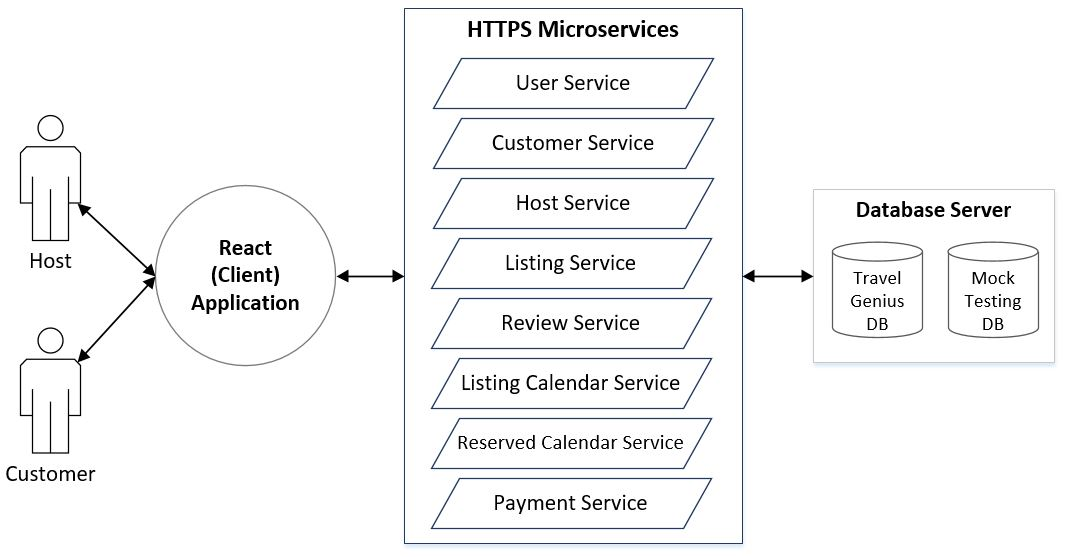
\includegraphics[width=0.5\textwidth]{../Architecture/Architecture.JPG}
		\caption{MVC Architecture for Travel Genius Project} \label{fig_1}
	\end{figure}

    This is not structuring just for the sake of adhering to good practices. It has a crucial future application aspect to our project. For example, consider:
    \begin{itemize}
        \item \textit{User Authentication:}  This is usually performed via different services, and can take multiple forms such as OTP, fingerprint, authApp , etc.
        \item \textit{Payment Service:} It is ideal to be facilitated via an isolate Payment Gateway.
    \end{itemize}
    
    Such updates, when required, can be made easily with minimal changes in the client application. Also, the micro-services mostly work in isolation, thus adhering to low coupling and high cohesion. The responsibilities, with respect to this architecture, have been divided as follows:
    \begin{itemize}
        \item {\textbf{DB Design, Data Mining:}  Nirav, Uditya}
        \item {\textbf{Microservices (REST APIs):} Uditya}
        \item {\textbf{Front End (React Application):} Nirav}
    \end{itemize}
 
\section{\textbf{Entity-Relationship (ER) Model}}
    \begin{figure*}[t]
        \centering
		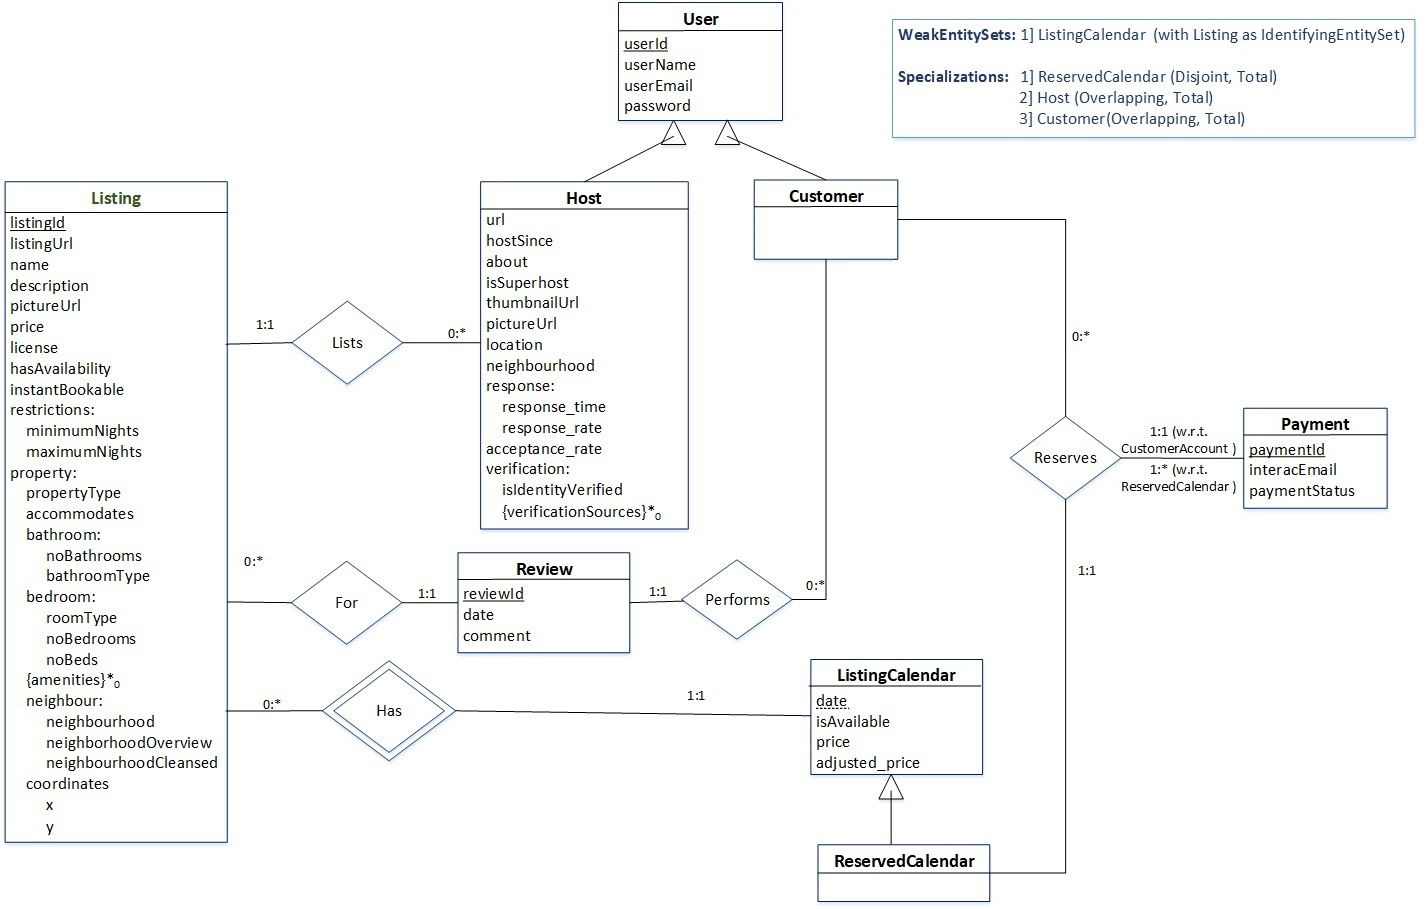
\includegraphics[width=1\textwidth]{../ER_Model/ER_Model.JPG}
		\caption{Entity-Relationship (ER) Model} \label{fig_2}
	\end{figure*}

\subsection{\textbf{Dataset Breakdown}}
\textbf{Fig-\ref{fig_2}} shows the Entity-Relationship model that was created on the basis of multiple observations made in the dataset. The original dataset \cite{1_Airbnb} has 3 files in any region - namely ‘reviews’, ‘listings’ and ‘listingCalendar’.
    \begin{itemize}
        \item ‘listings.csv’ \cite{1_Airbnb} alone contains over 50 attributes on its own. This is where we get information related to \textbf{Listings} and \textbf{Hosts}.
        \vspace{1mm}
        \item None of the datasets cover customer entity in full. However, the reviews dataset does contain the name and id of the customers (who had written the corresponding review). Hence, even though this need-not cover all the customers, still it can be utilized to a large extent. Hence, ‘Review’ and ‘Customer’ entities are created on the basis of data in ‘reviews.csv’ \cite{1_Airbnb}.
        \vspace{1mm}
        \item Data in ‘ListingCalendar.csv’ helps create \textit{‘ListingCalendar’} and \textit{‘ReservedCalendar’} entities.
    \end{itemize}

\subsection{\textbf{Some interesting design choices}}
    In this section, we cover some of the interesting design choices we had to make while creating the relational model and the explanation behind those choices.
    \begin{enumerate}
        \item \textit{User, Host, Customer}
    	    \begin{itemize}
                \item Host (implied by ‘Listings.csv’\cite{1_Airbnb}) and Customer (implied by ‘Reviews.csv’\cite{1_Airbnb}) contain 2 attributes in common - ‘id’ \& ‘name’. Hence, we create a Total Generalization on them.
                
                \vspace{1mm}
                
                \item  \textit{Why an Overlapping Generalization?}  The use-case for our application is such that only Customer-Accounts can make reservations and perform reviews. However, careful observation of the data shows that some host id(s) also exist as reviewerId(s) in ‘Reviews.csv’\cite{1_Airbnb} -  which means that Hosts can also be Customers (and vice versa).
                
                \vspace{1mm}
                
                \item \textit{userEmail:} This is not readily available in the data set. However, it forms a crucial part of our application, as majority of the communication with users is expected to happen via email.
                Hence, we make this field nullable as of now, and allow for existing users to update their email-ids. Any new account going forward must have an email-id. Another aspect of this is with respect to login, which we will discuss in section \textbf{\color{red} \textbf{Section-\ref{sec_userApplication}}}.
                
                \vspace{1mm}
                
                \item \textit{Why no specialization for VerifiedHost?  Aren’t ‘verificationSources’ only available for VerifiedHosts?}\\
                    \textbf{\color{green}No!} - ‘verificationSources’ are even available for records where ‘isIdentityVerified = false’. Hence, to a first guess, it is likely the case that ‘verificationSources’ also contain the sources from failed attempts.

		\vspace{1mm}

		\item \textit{Host has a field 'isSuperHost'? Wouldn't this imply a recurring relationship ?}\\
                    \textbf{\color{red}Yes!} - It must. However, to have such a relationship, we need the superHostId for all Hosts who are not superHosts. But this data is not made available in the dataset. Hence we are not considering this aspect in our project at this point.

            \end{itemize}

        \vspace{1mm}
        
        \item \textit{Listing, ListingCalendar, ReservedCalendar}
            \begin{itemize}
                \item \textit{Why is ListingCalendar a weak entity set on Listing ?}\\
                {\small ‘ListingCalendar.csv’\cite{1_Airbnb} contains the multiple availabilities that were created for an existing \textbf{‘Listing’}, where ‘date’ (in combination with ‘listingId’) forms the unique identifier.}
                \vspace{1mm}
                \item \textit{In the given dataset, how can we identify records for the specialization ‘ReservedCalendar’?}\\
                   \textbf{ ‘isAvailable = false’ could mean 3 possibilities:}
                    \begin{itemize}
                        \item \textbf{CASE-I:} All such listingCalendar(s) have been explicitly made unavailable by the ‘host’.
                        \item \textbf{CASE-II:} All such listingCalendar(s) have been reserved by different customer(s).
                        \item \textbf{CASE-III:} Some of such listingCalendar(s) have been explicitly made unavailable by the ‘host’, and some have been reserved by different customer(s).
                    \end{itemize}
    
                    \vspace{1mm}
                    
                    In the current dataset, there appears to be no way to know which of the 3 cases stand true. Hence, we make the following reasonable assumption and inference:
                        \begin{enumerate}
			  \item \textit{(isAvailable = ‘false’)} 
                                    \vspace{-7mm}
                                \[\Leftrightarrow \] \\
                                
                                    \vspace{-12mm}
                                \textit{(listingCalendar  isA  reservedCalendar)} 

                            \item If host explicitly wants to make a listingCalendar unavailable, then that listingCalendar is removed
                        \end{enumerate}
            \end{itemize}

	\item Payment
	    \begin{itemize}
	       \item Just like Customer and ReservedCalendar, Payment is also not readily available in the datasets.
	       \item However, for our use-case, we want to facilitate prepaid payments before confirming a reservation. Hence, we introduce a new table to allow this feature.
	       \item But we keep the option open, to change the implementation to a dedicated Gateway-based payment (for likely future changes), in which case the paymentId in ‘Reserves’ relationship-set will then also come from a remote external entity.
    	   \end{itemize}
     \end{enumerate}

    \vspace{-2mm}
 
   \subsection{\textbf{Summary}}
	   \begin{itemize}
	       \item We have 2 types of \textit{Users} (\textit{Customers} \& \textit{Hosts}).
	       \item A \textit{Host} can have multiple \textit{Listings}. Each listing can be made available for different dates (stored as \textit{ListingCalendar}). A \textit{ListingCalendar} (with current \& future dates) can be reserved by a \textit{Customer}, by making the required prepaid \textit{Payment}. All the reservations are marked with 'isAvailable = false' in \textit{ListingCalendar} and also have a corresponding entry in \textit{ReservedCalendar}.
	       \item A \textit{Customer} can perform \textit{Reviews} on past/current \textit{Reservations}.
    	   \end{itemize}

\vspace{-2mm}

\section{\textbf{Relational Schema}}
    Now we translate the above ER model to a relational schema, that can be utilized by client application(s) via the REST APIs. A reverse-engineered depiction of the relational schema (in MySql) has been shown in \textbf{Fig-\ref{fig_3}}.

   	 \begin{figure*}[t]
       		 \centering
		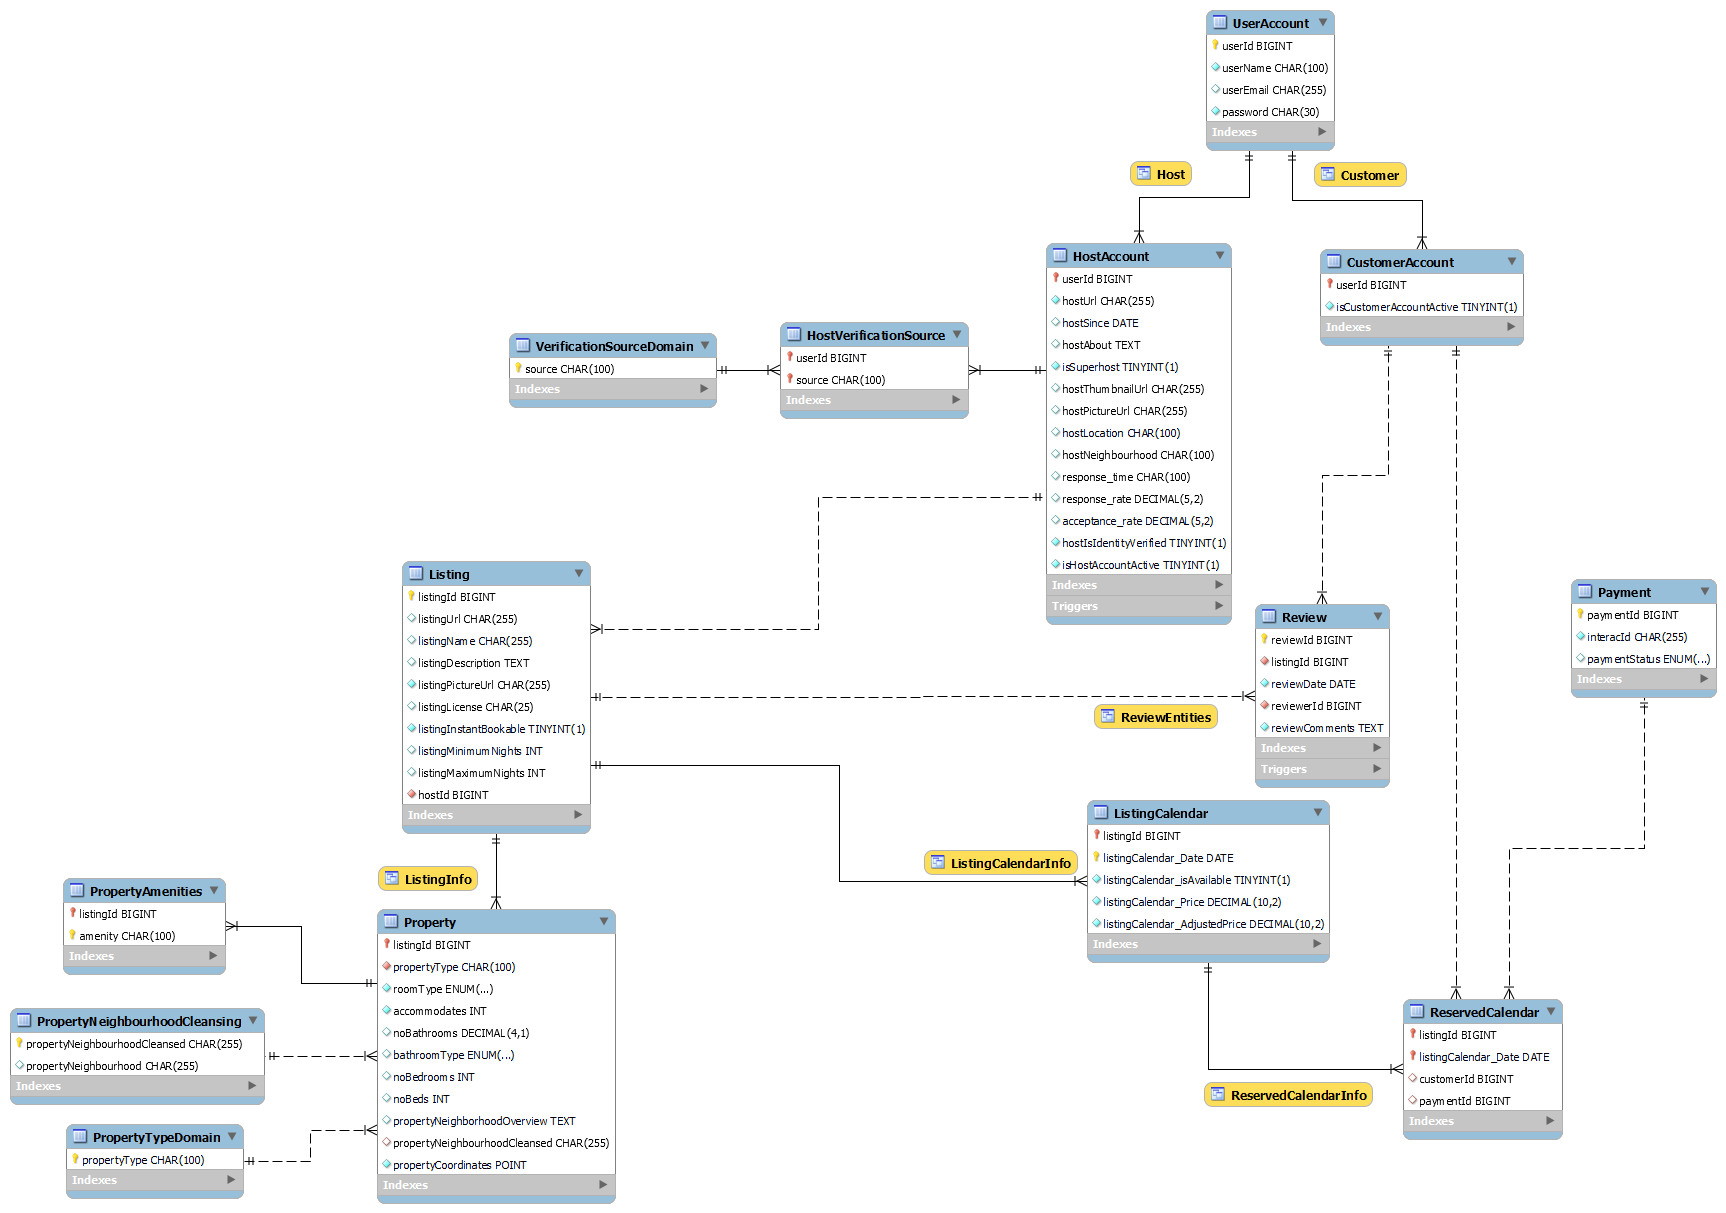
\includegraphics[width=0.95\textwidth]{../Relational_Model/RelationalModel.png}
		\caption{Reverse Engineered depiction of Relational Model for Travel-Genius in MySql} \label{fig_3}
	\end{figure*}


\subsection{\textbf{Some important observations}}
	\begin{enumerate}
	    \item \textit{Property as a Separate Relation}\\
	        Although, this was not required (as it had a 1-to-1 relationship with ‘Listing’ and was not resulting in any uncontrolled duplication), still we reallized that having such a large composite attribute as a separate entity would potentially make for more a adaptable design for (potential) future use - [E.g. if a future use case requires us to allow multiple listings for a particular property]
	    
	    \vspace{1mm}
	    
	    \item \textit{Multi-valued Attributes}
	        \begin{itemize}
	            \item \textit{verificationSources(Host)  \&  amenities(Property)} are the only 2 optional multi-valued attributes in the schema.
	            \item Hence we maintain them in separate tables with their individual value(s) and the corresponding (original) relation's Primary Key. The combination of the 2 acts as the Primary Key for the new relation.
	            \item We parse and process the array using Stored Procedures, which have been discussed in detail in next subsection.
	        \end{itemize}
	
	    \item \textit{Domain Correctness}
	        \begin{itemize}
    	            \item \textit{‘verificationSources(Host)’} currently holds values from among [‘phone’, ‘email’, ‘photographer’, ‘work\_email’]. Hence we maintain a foreign key relation to a separate domain table \textit{\textbf{‘VerificationSourceDomain’}} for this attribute.
    	            \item \textit{'paymentStatus(Payment)’}  holds values from among ['Pending', 'Completed', 'Cancelled', 'Refunded']. An enum has been used here to enforce domain correctness.
	        \end{itemize}
	
	        \vspace{1mm}
	
	\par
	        \textit{- Why is the domain correctness performed differently for the two ?}
	        
	        \begin{itemize}
    	            \item \textit{paymentStatus} is something, for which we expect the domain to rarely change.
    	Hence, ENUM() which requires higher privileges for any change to be made, can be facilitated by the respective authority.
    	            \item \textit{verificationSources} on the other hand are different. These can take many forms, and have high potential for frequent changes.
	Hence, we want to allow other stakeholders also (with required DML privileges or maybe even via an interface) to be able to make those changes.
	        \end{itemize}

		\vspace{1mm}

        \par
	        \textit{- Categorical data in Property:}
         
                \begin{itemize}
    	            \item \textit{propertyType:} contains over 90 categories and new types show up with each new added region. Hence we maintain a separate relation for domain correctness.
                        \item For \textit{roomType} \& \textit{bathroomType}, though, we make use of enum().
	        \end{itemize}
 
	\end{enumerate}

\subsection{\textbf{Stored Procedures \& associated feature abstractions}} \label{sec_storedProcedures_and_associatedFeatureAbstractions}
    Fig-\ref{fig_4} shows some of the important stored procedures that we’ve defined in our relational database.
(Refer:  \textit{'backend\_travelgenius{\textbackslash}\_\_data\_\_{\textbackslash}2\_ViewsAndStoredProcedures' \cite{4_Backend})} for detailed Stored Procedure implementations)

   	 \begin{figure*}[!h]
        		\centering
		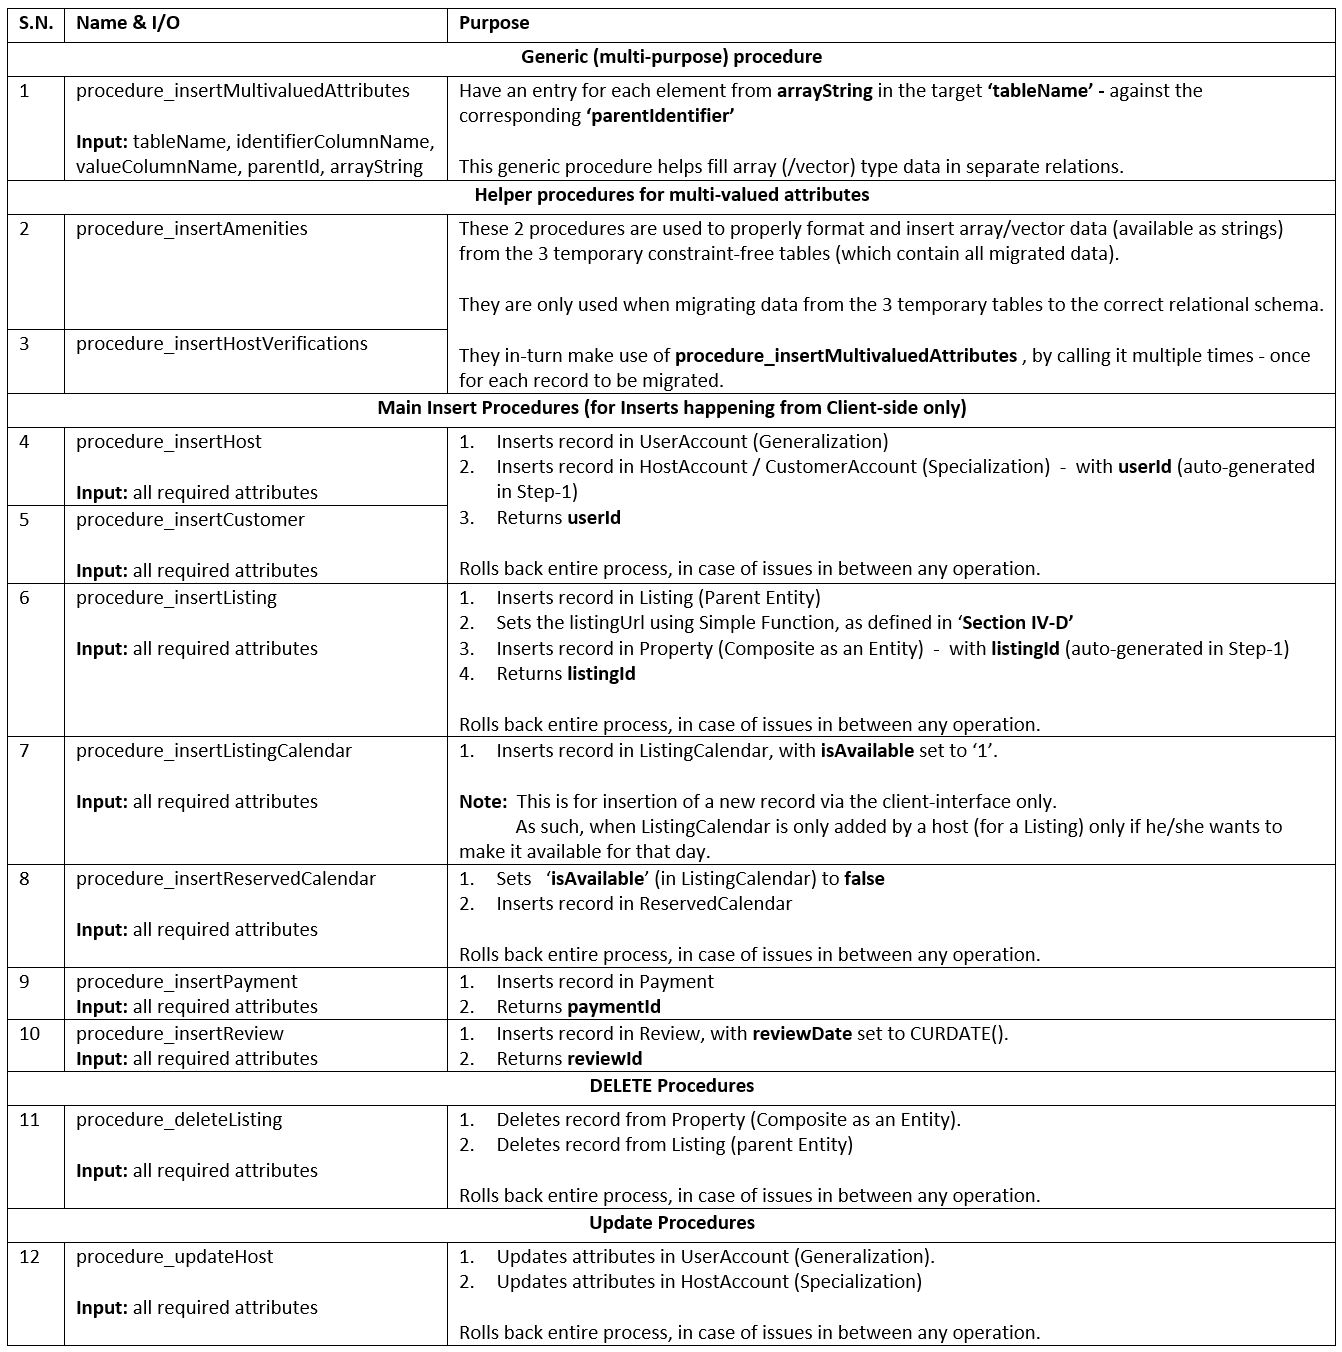
\includegraphics[width=1\textwidth]{../Directly_As_Images/StoredProcedures.JPG}
		\caption{Important Stored Procedures} \label{fig_4}
	\end{figure*}

    \vspace{1mm}
    
    \begin{enumerate}
        \item \textit{Why have these procedures, when a lot of these functionalities could have also been facilitated via the REST-APIs?}
            \begin{itemize}

                \item \textit{Need for database specific native Operations:}\\
                    E.g. Consider saving array type data in separate relations. For new records, added by client, this can surely be facilitated by the REST middleware.  \textit{But what about records added in bulk from large datasets ?}  \textrightarrow.  This is where database native procedures like \textit{'procedure\_insertMultivaluedAttributes'} are really useful.

		\vspace{0.5mm}

                \item \textit{Rollbacks:} Transaction Management can be handled much more easily with stored procedures. Consider the previous example again. Constraint violation for one value, means that the system should undo inserts for all other values in that array (for the record in question) \textrightarrow. these can be handled much more efficiently with stored procedures (with less potential for making mistakes).
                \vspace{1mm}
                \item \textit{Multiple sequential operations:} Can be handled much more efficiently - natively via stored procedures, also with rollback benefits as discussed earlier.
            \end{itemize}

	\begin{table*}[t]\centering
	        \caption{Views \& Associated Abstractions}\label{tab_1}
	        \begin{tabular}{|l|l|l|}
	            \hline
	            \textbf{S.N.}   & \textbf{Name} & \textbf{Purpose} \\
	            \hline
	            1    & Host                 & \multirow{2}{*}{\begin{tabular}[c]{@{}l@{}}1. Inner Joins UserAccount and HostAccount / CustomerAccount\\ 2. User-password is omitted\end{tabular}}                                       \\ \cline{1-2}
	            2    & Customer             & \\ 
	            \hline
	            3    & ListingInfo          & \begin{tabular}[c]{@{}l@{}}1. Inner Joins Listing and Property (this is a one-to-one join) \\ 2. Left outer joins the result with PropertyNeighbourhoodCleansed \end{tabular} \\ 
	            \hline
	            4    & ListingCalendarInfo  & 1. Joins ListingCalendar and ListingInfo \\ 
	            \hline
	            5    & ReservedCalendarInfo & \begin{tabular}[c]{@{}l@{}}1. Inner Joins ReservedCalendar \& ListingCalendarInfo and Left-outer-joins with Customer \& Payment\\ 2. Only provides paymentStatus and id from payment (Omits confidential details) \\ 3. Note: The joins with Customer and Payment are LEFT OUTER Joins, since they might have missing data.\end{tabular} \\ 
	            \hline
	            6    & ReveiwEntities       & \begin{tabular}[c]{@{}l@{}}1. Reviews is extended to get associated hostId (for the corresponding Listing)\\ 2. The Goal is to have the identifiers for all entities involved\end{tabular} \\ 
	            \hline
	        \end{tabular}
      \end{table*}        
        \item \textit{Some important observations}
            \begin{itemize}
                \item We’ve used stored procedures, only where we saw fit - on the bases of above potential benefits. All other operations, have been directly performed via the REST API middleware.
                \vspace{1mm}
                \item \textit{Why have procedure\_insertPayment ?}\\
                    It’s true that this is a simple record insertion. But we had a procedure for every other potential insert that could happen in our application. Hence, we decided to have one for Payment as well, to maintain consistency.
            \end{itemize}

	    \item \textit{Some use-case specific omissions} \label{sec_someUsecaseSpecificOmissions}
	        \begin{enumerate}
	            \item \textit{Why no update/delete for listing ?}
	                \begin{itemize}
    	                    \item Listings have available and reserved days (ListingCalendar (with isAvailable = true) and ReservedCalendar respectively) associated with them. Any changes made to a listing have implications on the reservations for different days. Hence, we have decided to not allow updates to a listing, once it is created.

    	                    \vspace{1mm}

    	                    \item \textit{What if the host wants to have changes in a Listing for any future reservations ?}\\
    	                        This will have to be facilitated by creating a new listing for those availabilities \textrightarrow  by the Host.

    	                    \vspace{1mm}

    	                    \item \textit{Deleting an Availability: } is allowed  (directly implemented in the middleware)\\
    	                            \textit{Deleting a Reservation: } not allowed (unless cancelled by the customer)

    	                    \vspace{1mm}

    	                    \item \textbf{Note: } ‘Cancellation by Customer’ is not yet implemented in the application (due to time limitations), nor was it included in the initial proposal.
	                \end{itemize}

                \vspace{1mm}
	            
	            \item \textit{Why no delete for User (Host/Customer) ?}
	                \begin{itemize}
    	                    \item For this application, we are not allowing deletion of a user account. However, we do allow deactivation of individual Customer and/or Host account (not userAccount\textrightarrow since the specialization is overlapping)
    	                    \vspace{1mm}
    	                    \item \textit{Customer Deactivation: }  Allowed only when customer has no current/future reservations.\\
    	                        \textit{Host Deactivation: }  Allowed only when host has no listings with current/future reservations.
    	                    \vspace{1mm}
    	                    \item Both deactivations are handled by the REST APIs.
	                \end{itemize}
                 
	            \vspace{1mm}
             
	            \item \textit{Why no delete for Payment ?}
	                \begin{itemize}
    	                    \item A payment record must never be deleted. However, the status can be updated to Cancelled/Refunded (E.g. when a reservation is cancelled)
    	                    \vspace{1mm}
    	                    \item Reservation cancellation \& related Payment status update feature is not yet implemented though, as discussed earlier.
    	                    \vspace{1mm}
    	                    \item However, the database design is very well structured to incorporate these features in the future (as and when required).
	                \end{itemize}
                 
                \vspace{1mm}
	
	            \item \textit{Why no delete/update procedure for Review?}
                        \begin{itemize}
    	                    \item Was simple enough to be implemented directly via the REST middleware.
	                \end{itemize}
                 
                \vspace{1mm}
	
	            \item \textit{Why no update procedure for Customer?}
	                \begin{itemize}
    	                    \item A customer does not have any updatable attributes in CustomerAccount (accept for isCustomerAccountActive - which is deactivation specific). Hence, updating only UserAccount specific attributes was simple enough to be implemented directly in the REST middleware.
	                \end{itemize}
	        \end{enumerate}
    \end{enumerate}

    \subsection{\textbf{Views \& Associated Abstractions}}
        \textbf{Table-\ref{tab_1}} describes the views that we've created in the database. All these Views serve use-case specific purpose, in addition to protecting secure/confidential data. (For detailed implementation of these views, please refer: \textit{'backend\_travelgenius{\textbackslash}\_\_data\_\_{\textbackslash}2\_ViewsAndStoredProcedures.sql' \cite{4_Backend})}

        \begin{itemize}
            \item \textit{What about userAuthentication?}\\
		- We have a dedicated REST service for this.
            \item \textit{What about host verification?}\\
		- This feature is not yet implemented (as is consistent with initial proposal). But for any future implementation, we believe that it should have a dedicated REST service and will likely require remote calls to an external service for document verification.
        \end{itemize}

    \subsection{\textbf{Some notable constraints \& triggers (Other than Primary and Foreign Key Constraints)}}
        \begin{figure*}[t]
            \centering
            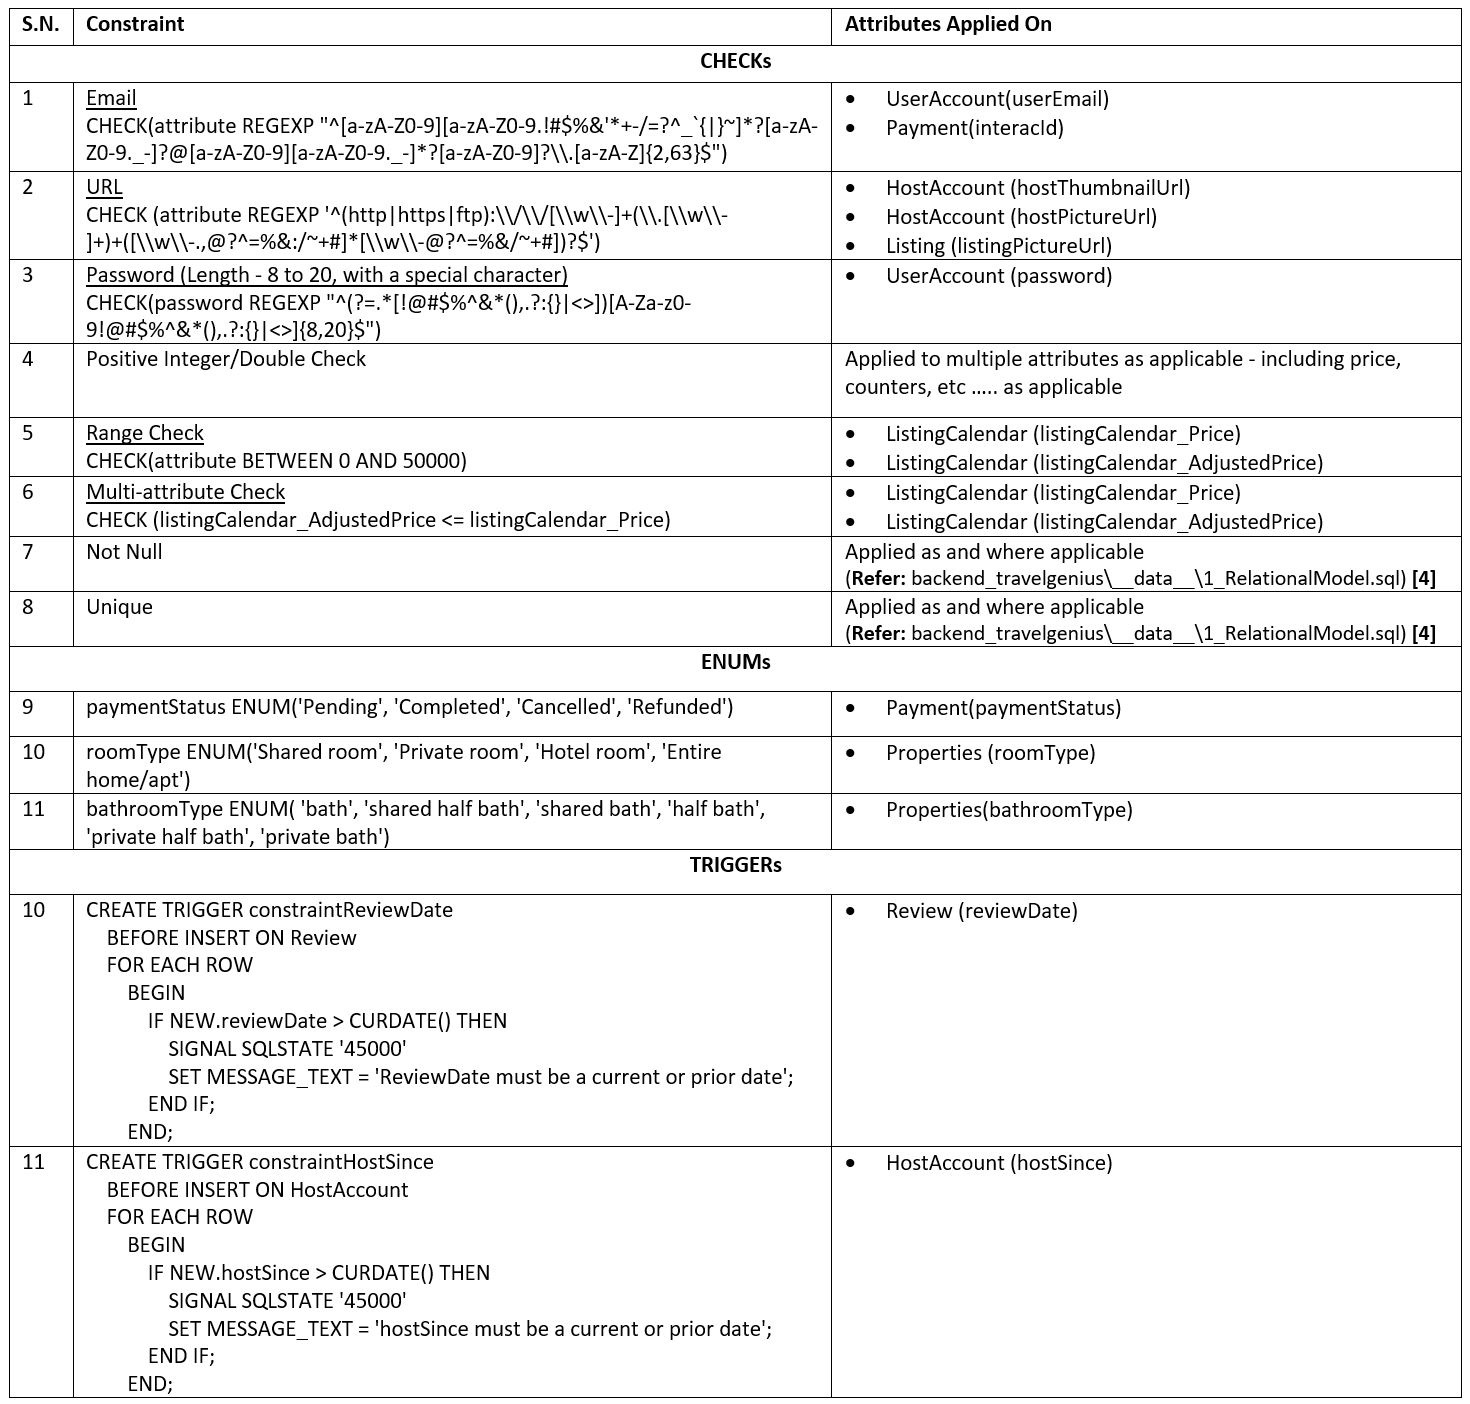
\includegraphics[width=0.9\textwidth]{../Directly_As_Images/Constraints.JPG}
            \caption{Some notable constraints \& triggers (Other than Primary and Foreign Key Constraints) \cite{2_Email_Regular_Expression} \cite{3_Regular_Expression}} \label{fig_5}
        \end{figure*}
        
        \textbf{Fig-\ref{fig_5}} lists some of these additional constraints. Note that we use a trigger for dates, since CURDATE() cannot be used in a CHECK constraint in MySQL.

        \vspace{1mm}

        \begin{enumerate}
            \item \textit{Simple Functions}
                \begin{itemize}
                    \item {\small hostUrl = concat('https:/www.airbnb.com/users/show/', userId)}
                    \item {\small listingUrl = concat('https://www.airbnb.com/rooms/', listingId)}
                \end{itemize}
    
            \vspace{1mm}
    
             \item \textit{Why not have a check-constraint/trigger to enforce this?}
                \begin{itemize}
                    \item {\small Since the identifiers have \textit{AUTO\_INCREMENT} property.}
                \end{itemize}
    
    	\vspace{1mm}
    
             \item \textit{How else are we enforcing this ?}
                \begin{itemize}
                    \item The inference on these Simple Functions was made after observing that the records in the dataset imply this.
                    \item Now, we need to ensure that any new records being inserted in the future do not violate this constraint.
                    \item We do this by having ‘Stored Procedures’ (Refer \textbf{Section-\ref{sec_storedProcedures_and_associatedFeatureAbstractions})} for inserting new Hosts and Listings, wherein the url is created and populated by the respective procedure after the Id is made available to it (via previous insertion).
                \end{itemize}

	\vspace{1mm}

	\item \textit{Why do we have PropertyNeighbourhoodCleansing relation ?}
 
                We need this relation to make sure that the following functional dependency (from Property) is not violated:
                
                 { 
                    \begin{center}
                        \footnotesize \textbf{\textit{propertyNeighbourhoodCleansed}  \textrightarrow} . \textbf{\textit{propertyNeighbourhood}}
                    \end{center}
                 }

	\vspace{1mm}

        \end{enumerate}

    \subsection{\textbf{Indices}}
        The use-cases for our application were such, that most of the operations already had the required indices in place due to the presence of relevant primary keys and foreign keys as required.
However, there is one complex query (for Searching Listings) that required more indexes. Every filter in that query is range-based; hence a B+ tree a good option for it. The dynamic implementation of the query in node.js has been shown in \textbf{Fig-\ref{fig_6}}.
Further, user authentication queries (point queries) also require 2 additional indexes.
        \begin{figure*}[t]
            \centering
            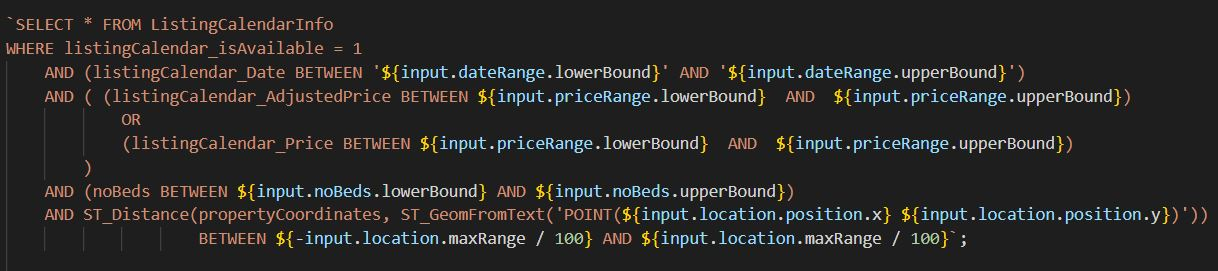
\includegraphics[width=0.9\textwidth]{../Directly_As_Images/SearchQuery.JPG}
            \caption{Search Query} \label{fig_6}
        \end{figure*}

        After doing analysis with ‘explain’ and ‘explain analyze’, the following indexes were found to be the most efficient and feasible:
	\begin{enumerate}
		\item \textit{Search Query}
  
		            CREATE INDEX\\
		            index\_listing\_isAvailable\_date\_price\_ListingCalendar ON\\ 
			     ListingCalendar ( listingId, \\
                  listingCalendar\_isAvailable,\\
				 listingCalendar\_Date,\\
				 listingCalendar\_Price,\\
				listingCalendar\_AdjustedPrice);

		\item \textit{UserAuthentication Queries}
			\begin{itemize}
                    			\item CREATE INDEX index\_listing\_userId\_password ON UserAccount(userId, password);
				\item CREATE INDEX index\_listing\_userEmail\_password ON UserAccount(userEmail, password);
			\end{itemize}
	\end{enumerate}

\section{\textbf{User Application}}\label{sec_userApplication}
    {We’ve already briefed the features that our application supports on Page 1, followed by the high level system architecture. All those features have been implemented via a React based User Interface. Fig \ref{login_form}, \ref{search_output} and \ref{manage_listing} show screenshots of log in page, search output, and Listings Management. Fig \ref{date_selection} presents date selection page to book any property. These are only for a small subset of the features that have been implemented. The entire suite of implemented features has been well demonstrated in the video. We've used a template from the internet to create this react interface.

    \begin{figure}[!h]
        \centering
        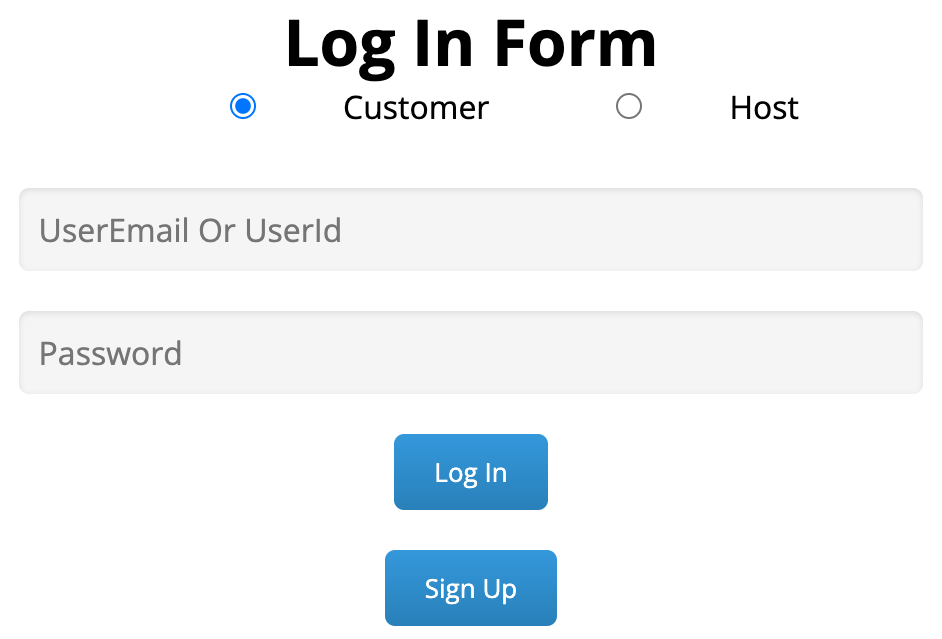
\includegraphics[width=0.3\textwidth]{../Directly_As_Images/loginform.png}
        \caption{Login form} \label{login_form}
    \end{figure}

    \begin{figure}[!h]
        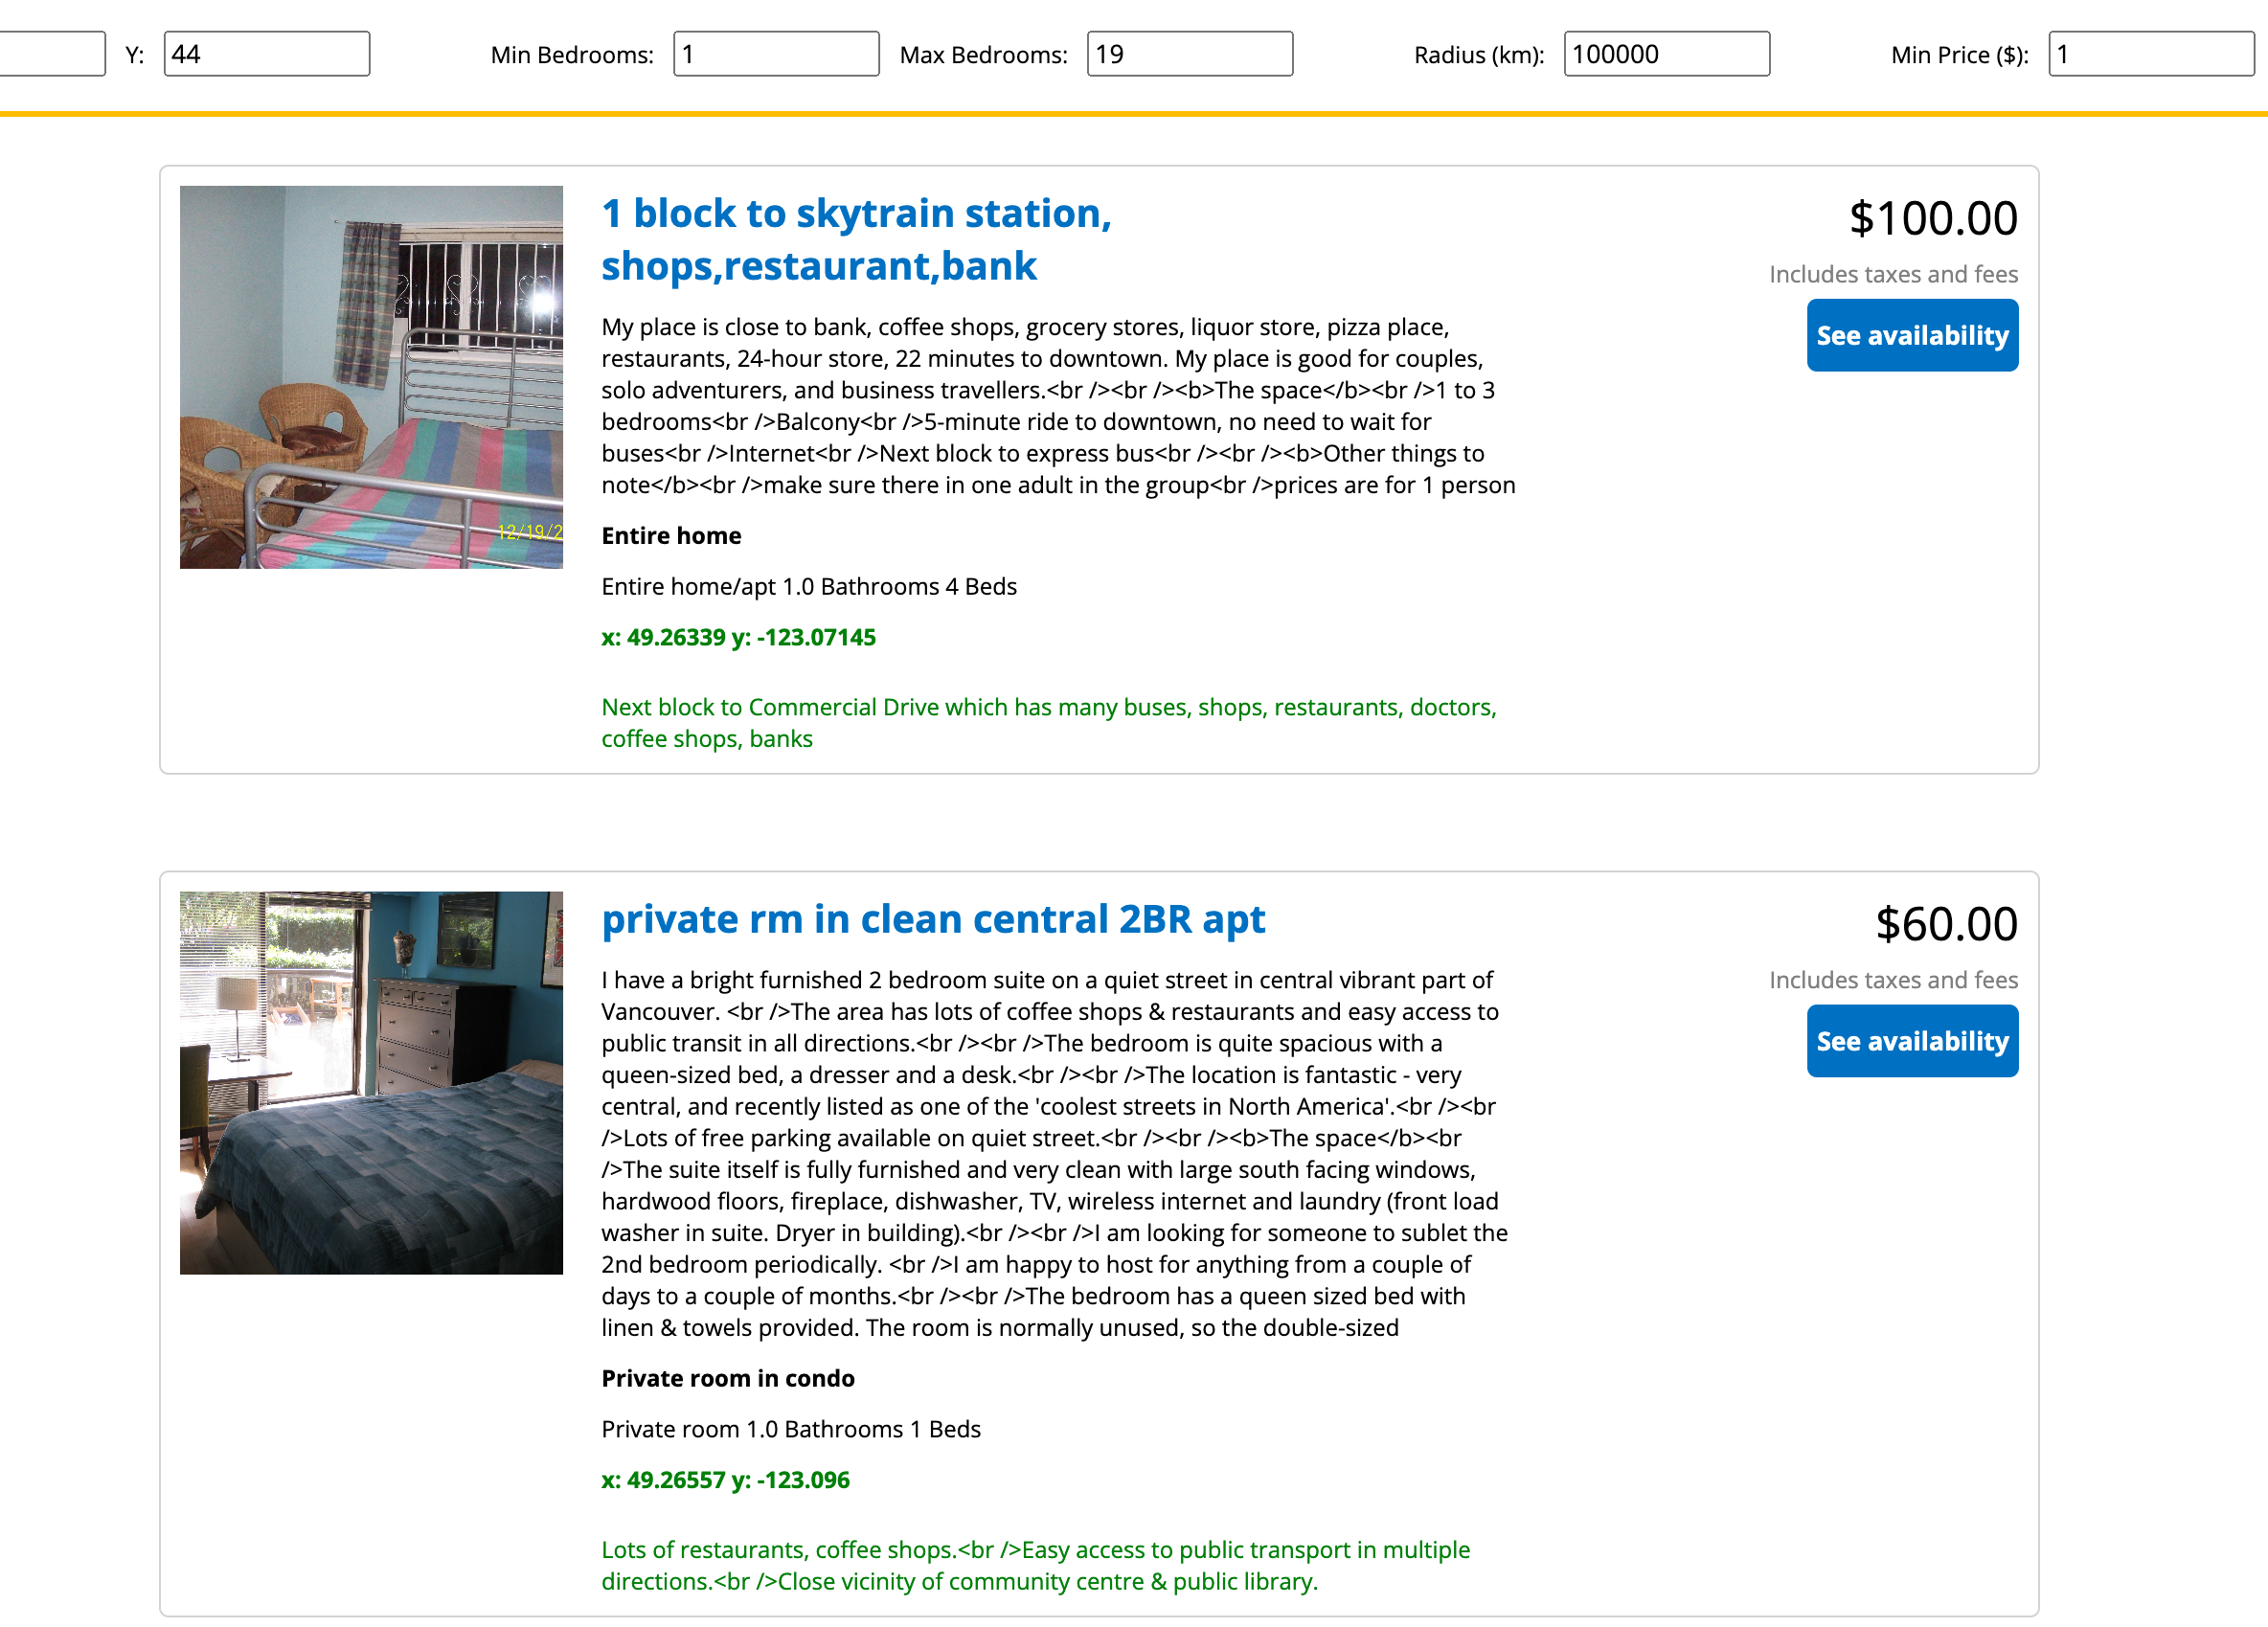
\includegraphics[width=0.35\textwidth]{../Directly_As_Images/search_output.png}
        \caption{Search Output} \label{search_output}
    \end{figure}

    \begin{figure}[!h]
        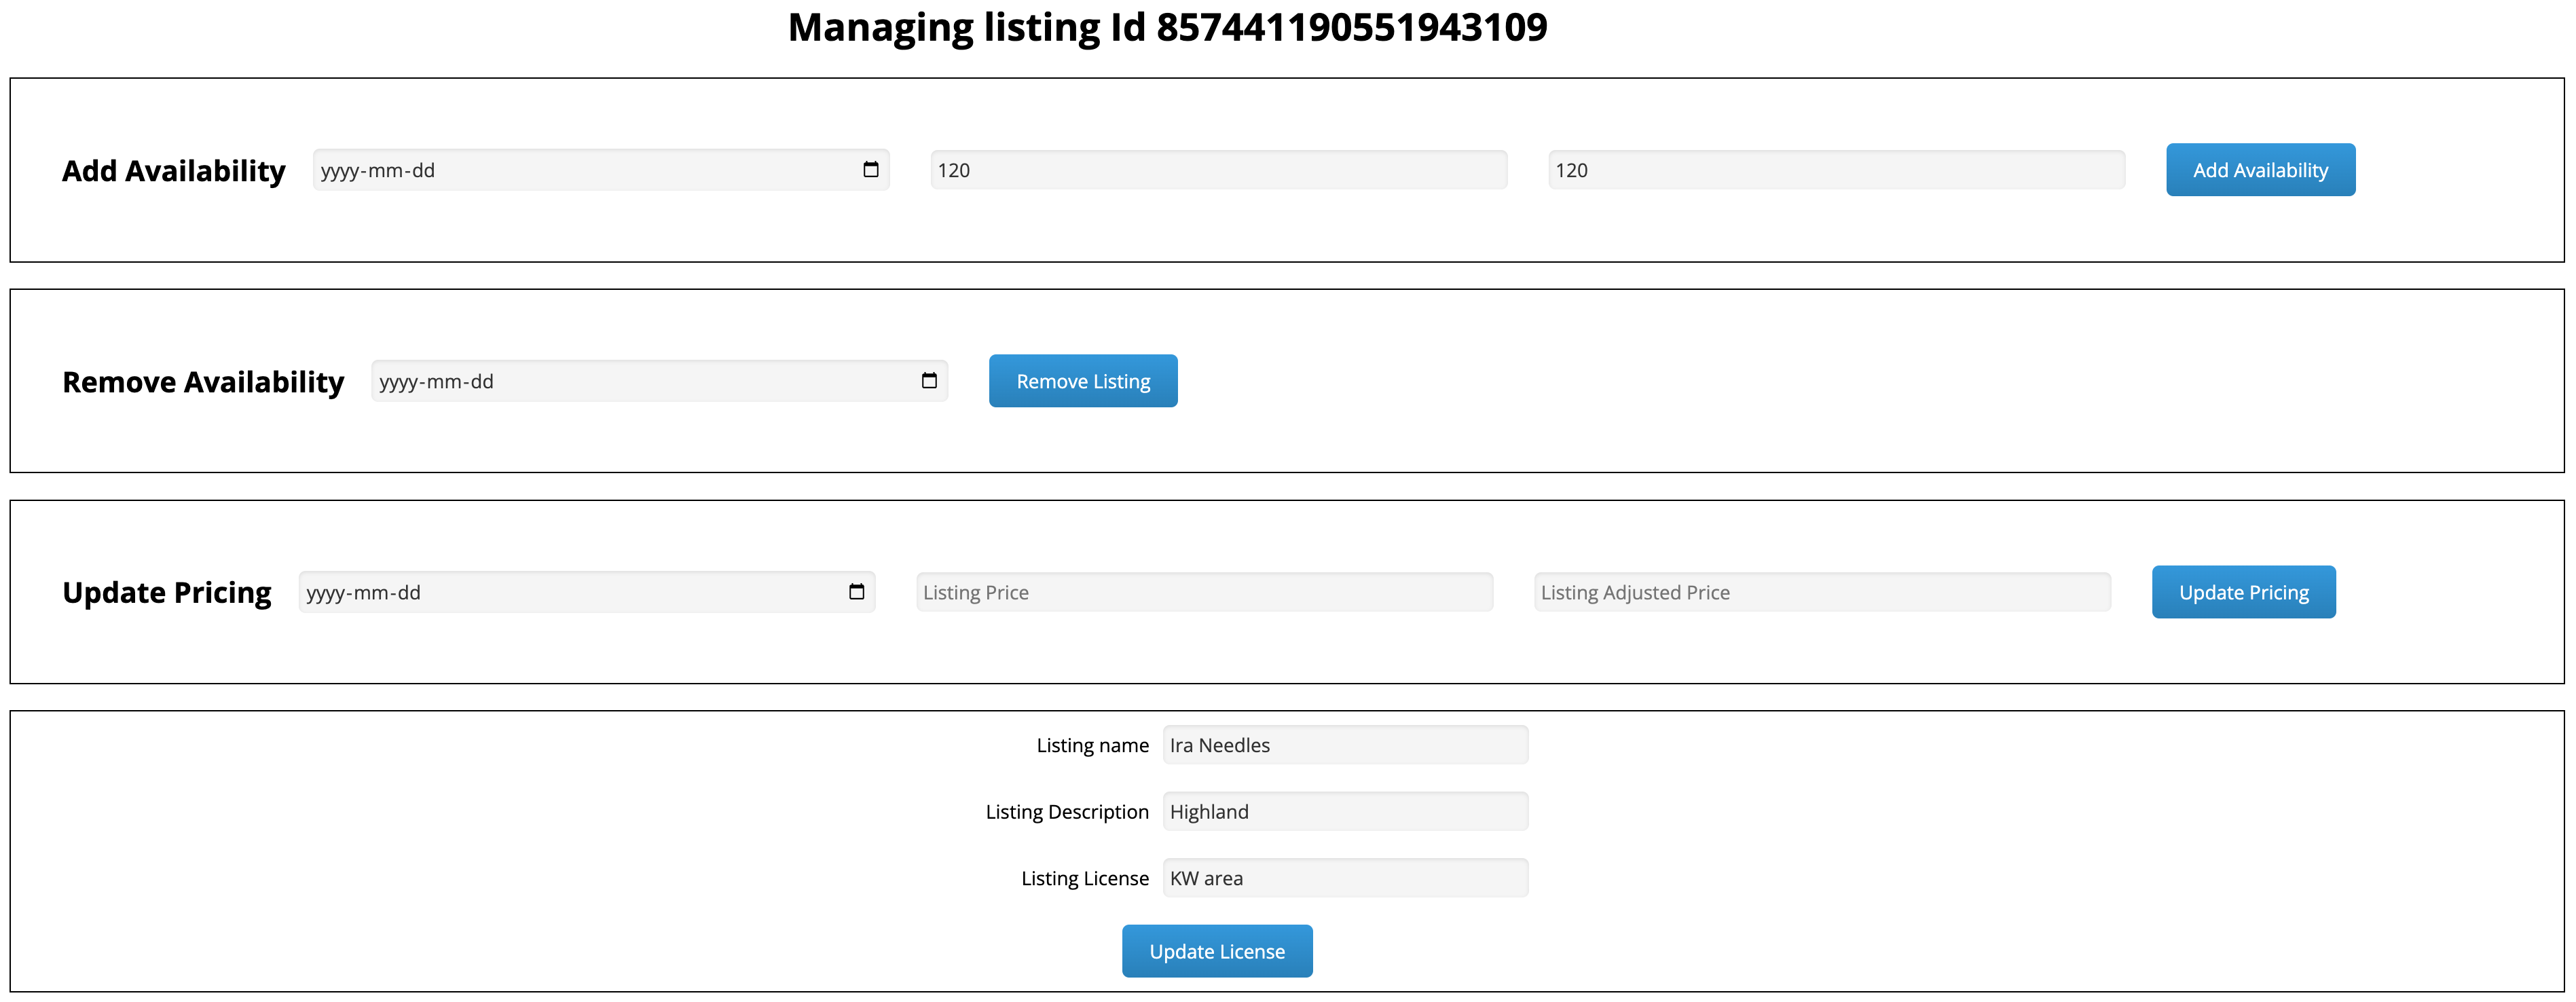
\includegraphics[width=0.4\textwidth]{../Directly_As_Images/manage_listing_host.png}
        \caption{Manage Listing} \label{manage_listing}
    \end{figure}

    \begin{figure}[!h]
        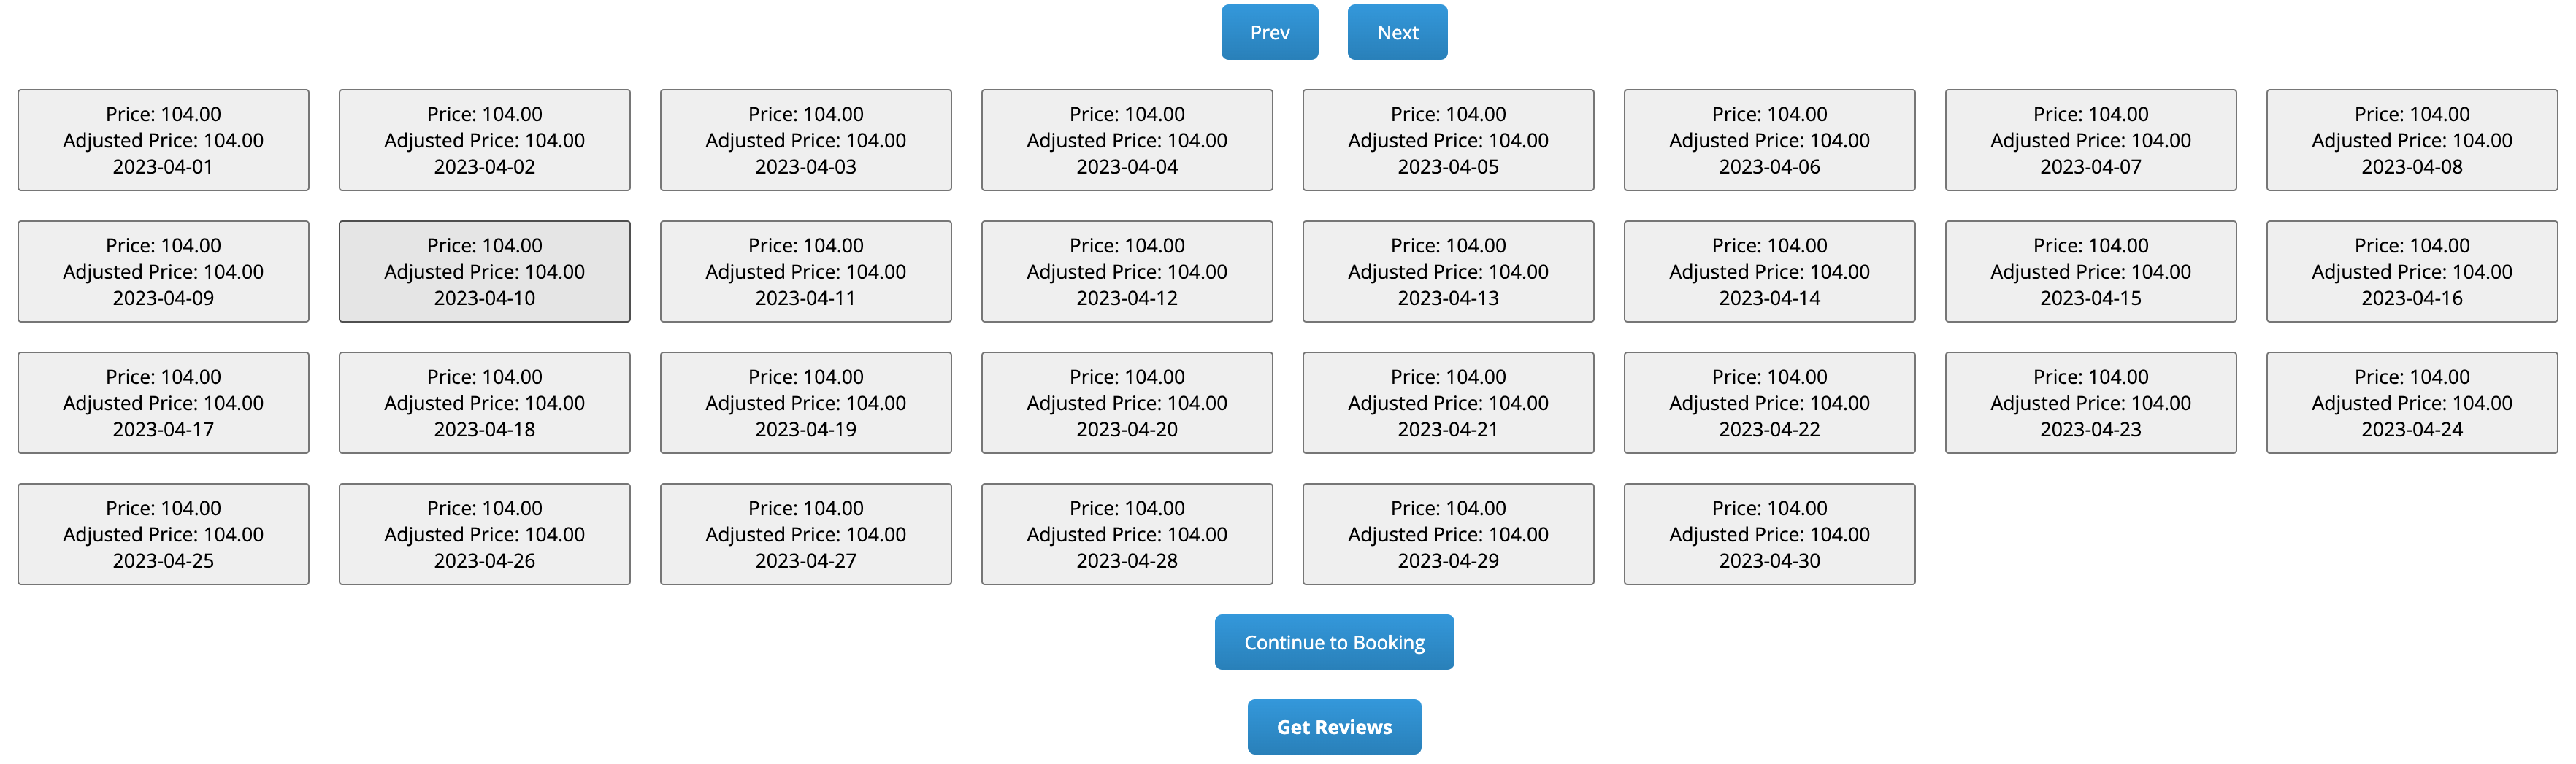
\includegraphics[width=0.4\textwidth]{../Directly_As_Images/booking_step.png}
        \caption{Date Selection during booking step} \label{date_selection}
    \end{figure}
    

\section{\textbf{Testing}}
    \subsection{\textbf{REST APIs Testing}}
        The test suites for REST APIs are fully automated via the \textbf{‘Mock Testing DB’}, which is a short lived, temporary database with dummy data and essentially the same schema as the original one. Hence, in addition to the REST APIs, the unit tests also end up testing several aspects of the database design.

	\begin{figure}[!h]
            \centering
            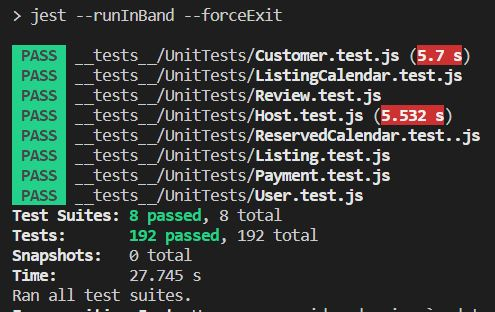
\includegraphics[width=0.35\textwidth]{../Directly_As_Images/REST_API_UnitTests.JPG}
            \caption{REST APIs - Unit Tests (Sample Run)} \label{fig_6}
        \end{figure}

        We use JEST Framework for the test setup. To view the complete test-setup, one can refer the following set of files in REST APIs (Backend\_TravelGenuis):
        \begin{enumerate}
            \item \textit{\textbf{./test\_setup.js:}}  which is the configuration that is run at the start of each test-file implementation
            \item \textit{\textbf{./Config/\_\_mocks\_\_/dbProperties.js:}}   Directs test framework to use (mock \& temporary) testTravelGenius database (created in test\_setup.js) instead of the real database.
            \item \textit{\textbf{./\_\_tests\_\_/MockData/3\_LoadData.sql:}}   (run in test\_setup.js)  Adds dummy (but relevant \& feasible) data to mock database, to perform testing on.
            \item \textit{\textbf{./\_\_tests\_\_/UnitTests/$<$filename$>$.test.js:}}  Each file in this directory is a dedicated test implementation for the corresponding service \& contains multiple test-suites for the same.
        \end{enumerate}
        
        The entire test-setup can be verified by running \textit{\textbf{`npm test`}} command from the parent directory of \textit{\textbf{Backend\_TravelGenuis}}

	



    \subsection{\textbf{Front-end Testing}}
        {The front-end application has been manually tested and the detailed test suite implementation has been provided in \textbf{\textit{'ece656\_frontend / FrontendTests.xlsx’}}. Considering the constraint in terms of time and resource, we have restricted ourselves to manual testing only.}

        Fig. {\ref{FrontendTests}} a screenshot for one of the test-suites. Remaining test-suites can be found in the corresponding tabs as marked below.
        \begin{figure}[!h]
            \centering
            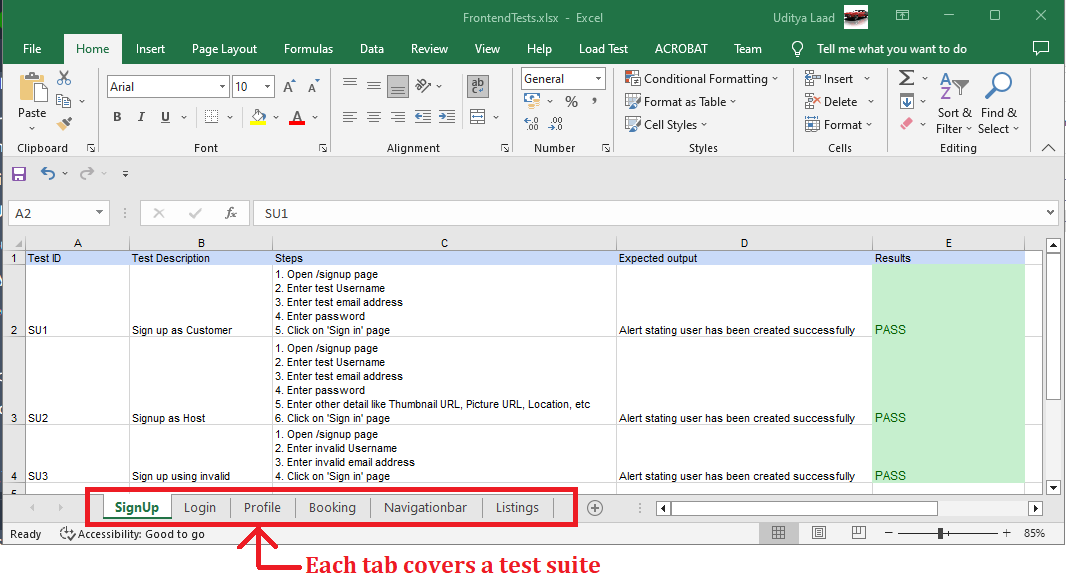
\includegraphics[width=0.5\textwidth]{../Directly_As_Images/FrontendTests.png}
            \caption{Front-end Manual Testing (Each Tab covers a test-suite)} \label{FrontendTests}
        \end{figure}


\section{\textbf{Data Mining Exercise}}
    \subsection{\textbf{Domain Appropriate Question:  What is the likelihood of success for a listing with respect to its features ?}}
	 \begin{itemize}
           	 \item \textit{Dependent Attribute: How do we measure success ?}\\
			We have 2 Relations ‘ListingCalendar’ (Availabilities for a listing on multiple unique days, which may also be reserved)  \&  ‘ReservedCalendar’ (ListingCalendar that are reserved by customers). Hence we define: \\

				$  SuccessRate(listingId)  =  \frac{| ReservedCalendar(listingId) |} {| ListingCalendar(listingId) | } $ \\ 
				
				Success Rate is not directly available as a field in the database. Hence, we trigger an SQL query to compute this field and associate it with the corresponding Listing features vis Jupyter Notebook. (The query and resulting CSV can be found in  \textit{'backend\_travelgenius{\textbackslash}\_\_datamining\_{\textbackslash}DataMining.ipynb' \cite{4_Backend}})

		\vspace{1mm}

		\item \textit{Independent Attibutes}\\
			Subset of features associated with listings (to be selected)
	\end{itemize}
        
   \subsection{\textbf{Technique(s) appropriate to the question}}
	The features associated with Listing are mostly dominated by categorical and numeric values. Note that fields like listingUrl, listingId, license are of no relavance here - since these essentially identifiers. Although, pictureUrl does indeed point to a hosted picture. However, due to time and resource limitation, we have decided not to pursue image processing  (\& will hence treat it under future scope for analysis).
	
	There are a lot of numerical attributes where the distribution is over a small range, hence potentially convertable to categorical data (ordinal or otherwise). However there are some others which cover a relatively larger range (e.g. price).

	\vspace{1mm}

	Now, given the nature of the question and the features to choose from, there are 2 potential model building techniques that we see fit:
	\begin{enumerate}
           	 \item \textit{Linear Regression: }\\ There is a possibility (although very low) of a linear relationship between the dependent and independent attributes. We can treat this as our NULL hypothesis, the results of which ill be clear at the feature selection stage, when performing correlation analysis.
		\vspace{1mm}
		\item \textit{Multi-Layer perceptron (MLP): }\\ There is a high chance that the relationship we are seeking is not linear. In such a case, linear regression is infeasible. MLP, on the other hand, provides the flexibility of building a non-linear model using multiple hidden layers with (specific) activation functions, as applicable to the situation.
	\end{enumerate}

	Note that the target value is probalistic (in range [0, 1]). This is the major reason behind potential selection of above 2 techniques, among other reasons - as will be discussed in the subsequent sections.

	More techniques to be considered for feature selection are:
	\begin{enumerate}
           	\item Correlation Analysis
		\item Checking Frequency Distribution
		\item Looking at potential use of Principal Component Analysis
	\end{enumerate}

   
     \begin{figure*}[t]
       	\centering
	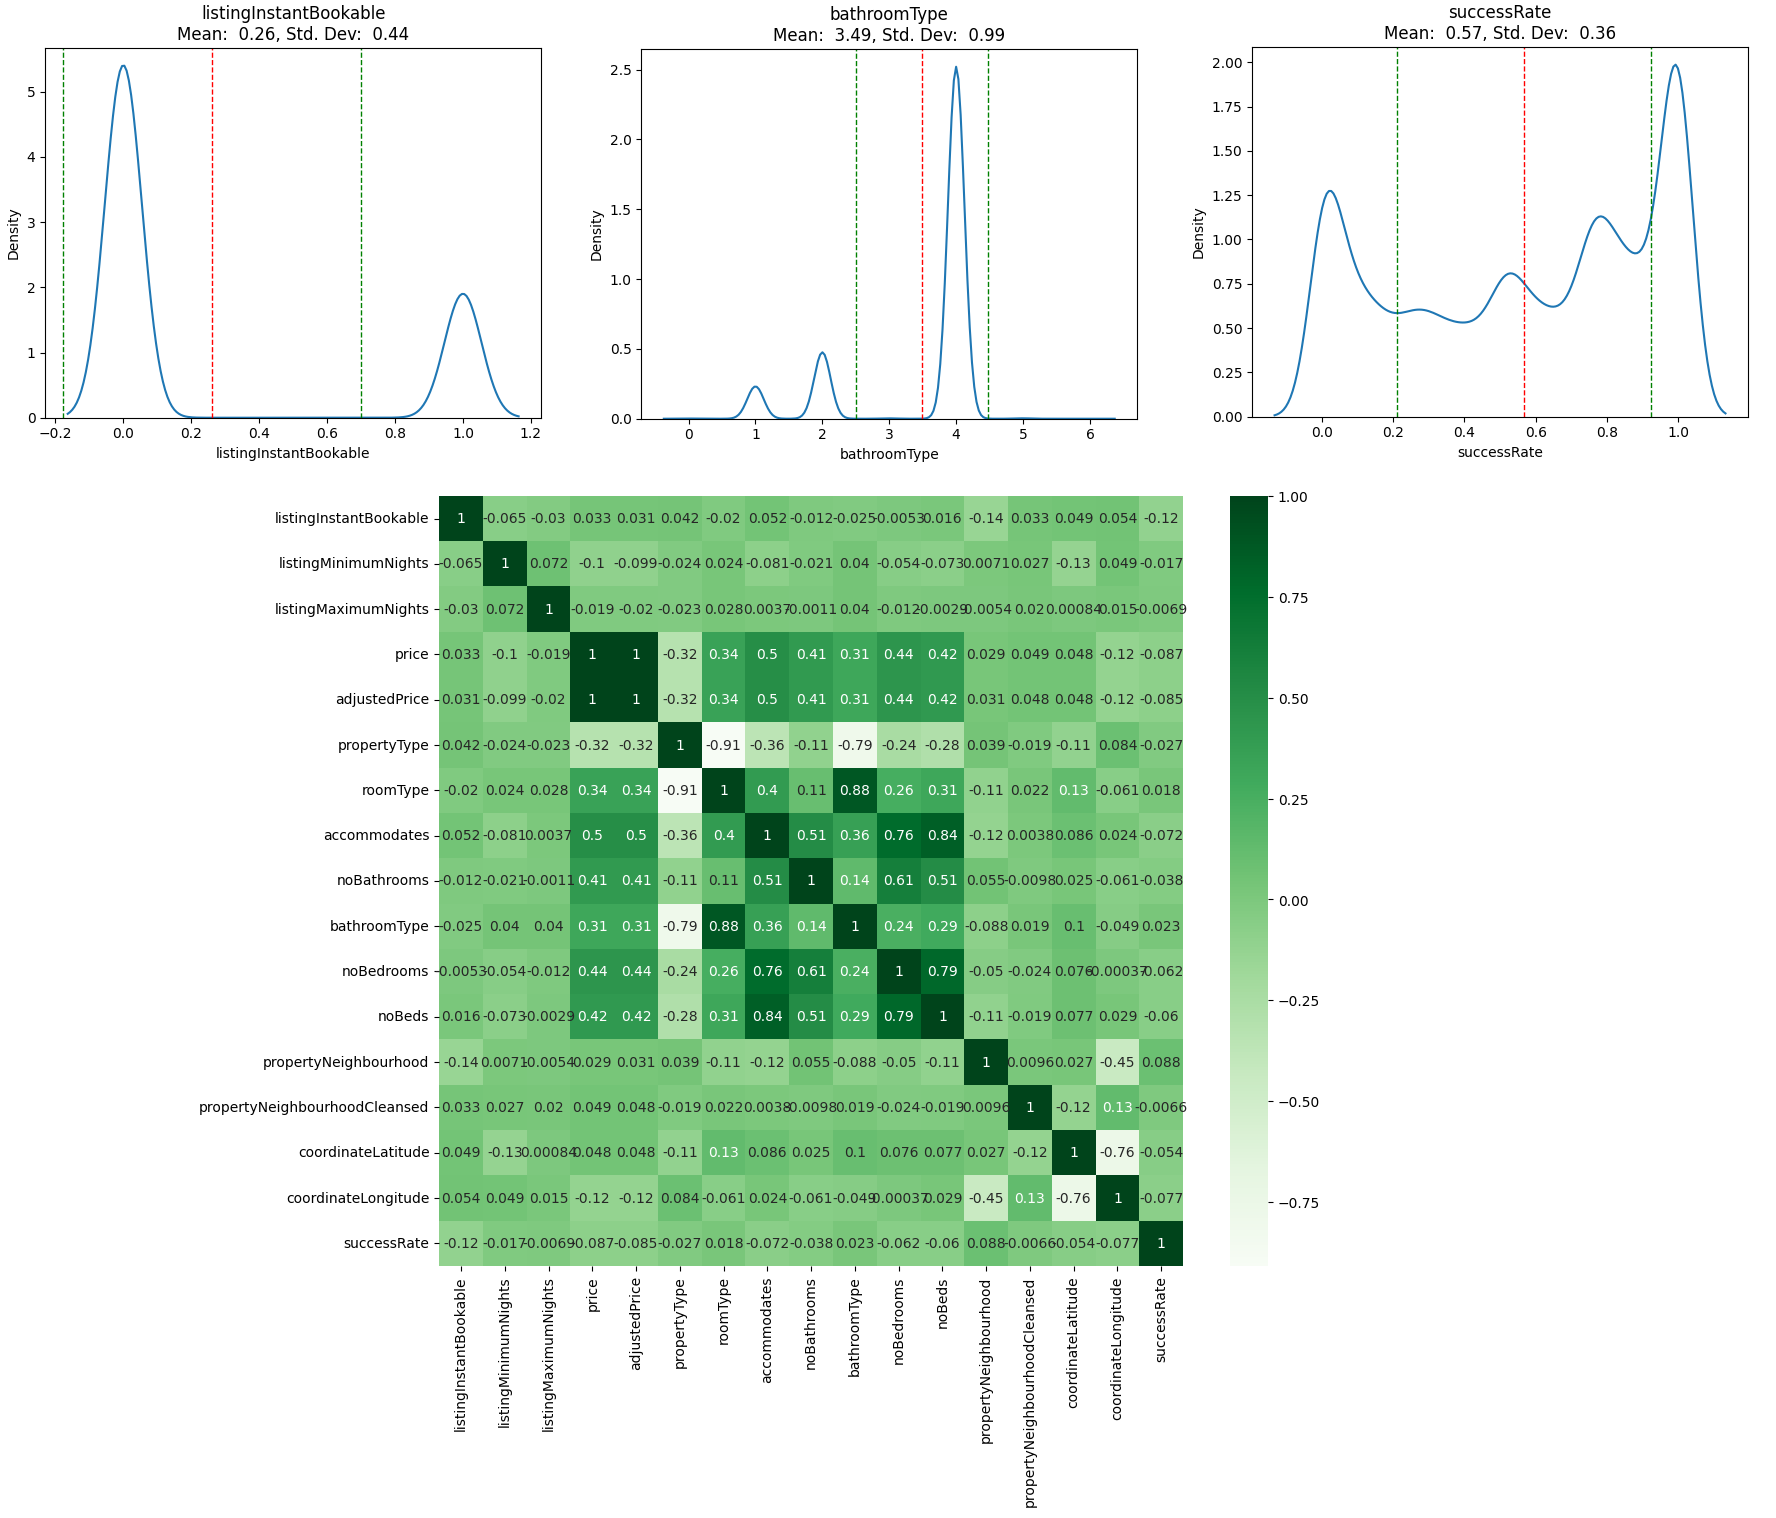
\includegraphics[width=1\textwidth]{../Data_Mining_Images/CorrelationAndFrequency.png}
	\caption{Frequency Distribution for 2 interesting attributes and Results of Correlation Analysis \cite{7_FeatureSelection}} \label{fig_7}
    \end{figure*}
	
     \subsection{\textbf{Pre-processing of Data}}
	Both the model-building techniques under consideration require features to be in numerical form. Having reasonably ommitted some features in step-1, we now look at some of the other features that require a look-in. For the first two attributes, we are \textit{\textbf{defining fuzzy boundaries}} to derive meaningful categories for them.
	\begin{enumerate}
           	\item \textit{roomType}\\
			This is categorical data. Close observation shows that we can inbibe meaning in the labels that we intend to assign for these categories. E.g. An entire home/apt is typically considered to be better than a Hotel room. As such these categories are comparable, giving us an opportunity to (somewhat) make them ordinal. Hence, we define and utlize the following mapping:
		 	 \textit{ \{ 'Shared room': 1,  'Private room': 2, 'Hotel room': 3, 'Entire home/apt': 4 \} }
		
		\item \textit{bathroomType}\\
			This is also categorical data. Consider the following mapping:
			\textit{ \{'private bath': 1, 'shared bath': 2, 'half bath': 3, 'bath': 4, 'shared half bath': 5,  'private half bath': 6\} }
			
			Ideally, most people would consider ‘Private-bath’ to be the best of the lot. However, consider the ‘bath’ cateogory. It does not tell much about anything - as such, considering it to be a neutral type looks like a reasonable assumption to make. Why ? Different individuals are likely to treat this differently. Some customer may find it skeptical, while others may ignore it.

		\item \textit{propertyType}\\
			This is categorical data that needs to be translated to meaningful numerical labels. For this purpose, we use Vectorization technique available under scikit learn. 

		\item \textit{\small propertyNeighbourhood  \&  propertyNeighbourhoodCleansed}\\
			These fields can be made categorical and will be meaningful with respect to proximity of location. However, we see that they are functionally dependent on propertyCoordinates. propertyCoordinates is likely to cover for any affect they might have on the successRate.
	\end{enumerate}


	
     \subsection{\textbf{Correlation Analysis \& Frequency Distribution}}
	Note: our feature selection process had already begun from step-1, when we gradually started eliminating certain features on the basis of reasonable arguments and/or techniques.
	We now look at the frequency distribution and correlation analysis chart (\textbf{Fig-\ref{fig_7}}) for better understanding of the relationships. For frequency distribution of all attibutes, please refer \textit{'backend\_travelgenius{\textbackslash}\_\_datamining\_{\textbackslash}DataMining.ipynb' \cite{4_Backend}}.
	
	As is evident from \textbf{Fig-\ref{fig_7}}, none of the independent attributes have an individual correlation coefficient greater than 0.5 with respect to the successRate. Such low collinearity values falsify our initial null hypothesis, which suggested that there exists a Linear Relationship between success rate and listing feaures (of importance).\\
	\textit{How can we still make use of correlation analysis?}  We also have frequency distribution and some more graphs to make certain inferences on feature selection. The middle portion of the correlation analysis signifies something intersting. There is high collinearity among some independent attributes (multi-colinearity). This can potentially mean that they act together in their effect on successRate. This however, is not an inference, but rather a logical observation by looking at the figures and types of attributes at play. The major point, being that, we cannot simply eleminate them due to low colinearity.

	

	\begin{itemize}
		\item \textit{What about price \& adjustedPrice ?}\\
The frequency distrbution seems to suggest no major differences between the two - \textit{Should we get rid of one of them ?} - No! Discounts often tend to occur in relatively smaller chunks; a small change in price may still have a big impact on the successRate, as is quite frequent with many discounted products.

		\item \textit{Frequencies for 2 interesting attributes:} isInstantBookable is a binary attribute and bathroomType is a categorical attribute. listingInstantBookable for one of the regions has a true:false frequency ratio of 1:6 with almost negligible correlation, which could lead one to believe that the value has no impact on the target and will be simply an overhead on the model builder. However, when multiple regions are taken together, the ratio raises to nearly 1:3 with a comparably higher (even though still low) correlation. A similar pattern can be seen with bathroomType here which has most values concentrated at 4. It also has a very low correlation with the target. There is no clarity on such 2 attributes at the moment, but considering their domain size and nature, we decide to keep them in our feature set.
	\end{itemize}

	After considering all the eliminations so far, we are now left with the following attributes in our feature set:
	\{ price, adjustedPrice, propertyType, roomType, accommodates, noBathrooms, bathroomType, noBedrooms, noBeds, listingMinimumNights, listingMaximumNights, propertyCoordinates(lat, long), listingInstantBookable \}

	\textit{Do we need Principal Component Analysis (PCA)?}\\
            PCA would have been useful if we had a comparatively large set of attributes, and also in case there was a particular need to pick relavant characteristics from the feature set.
            However, for a total of 11 independent attributes, with meaningful data distribution in most, dimensionality reduction does not make sense here. One attribute that we had to be carefull about was 'propertyType' as we had applied scikit based vectorization for it’s label encoding. But this is something, that MLP should be more than capable of handling with right configuration in place.


	\subsection{\textbf{Model Building using Multi-layer perceptron (MLP)}}
		\begin{itemize}
			\item We use Tensorflow \cite{6_MLP} to configure \& build our model.
			\item An MLP based model makes use of numerous hidden-layer nodes, each with their dedicated activation functions to allow non-learity in the model.
			\item\textit{ Choice of parameters:}\\
				\textit{Activation Function(s):} We tried 3 main activation functions in different configurations:
				\begin{enumerate}
					\item \textbf{relu} - due to its non-linearity, sparsity, ability to avoid vanishing gradient problem
					\item \textbf{sigmoid} - since the target is probabilitic \& since it also helps with input normalization
					\item \textbf{tanh} - since it is less prone to saturation than sigmoid\\
				\end{enumerate}

                \vspace{-2mm}

				\textit{Number of hidden layers:} due to the number of features involved, we initially though that 3 layers with gradually increasing neurons might serve well. However, 3 layers proved to be insufficient and we ended up using:  4 layers with (256, 512, 1028, 1028) neurons respectively. The initial parameters were decided on the basis of our experience with other neural networks in the past (for other courses).   We were expecting relu to be of particlular use here. However, the feature selection, and mapping turned out to be quite significant in being able to achieve such high accuracy with only sigmoid in place at each neuron.\\
				This was not straightfarward though. Initially, we made the mistake of assigning simple dataframe based labels for categorical data, which resulted in very poor accuracy. It was only after we devised the fuzzy boundaries and assigned meaningful labels for the attributes, that we were able to achieve the end results.

				\textit{Measure of Accuracy:} We use Mean-square-error as the measure, due to use of Sigmoid as activation function \& since it makes it easy to optimize gradient descent.\\
				\textit{Learning Optimization:} We use Adam - since it combines momentum and adaptive learning rates, to achieve faster convergence and better performance.
		\end{itemize}


	\subsection{\textbf{How model was validated ?}}
		The model was validated in 2 phases:
		\begin{itemize}
			\item \textit{During model building process - with Test Set Validation:} This was utilized during initial model creation process - to check the effectiveness of the built model, look for overfitting issues, etc
			\item \textit{K-Fold Cross Validation - Post model creation:} \\
				we validated our model thouroughly by performing K-fold validation with k = 5. The process was as follows:
				\begin{enumerate}
					\item Divide the input-set into 5 equally distributed test sets
					\item For each test-set 't' in input-set 'T':  Run the model builder with same properties; (T - t) as training set  \&  then validate the model against 't' 
					\item Compute the mean and standard deviation (of scores - in terms of Mean Square Error) for the 5 tests
					\item Compare results to assess the model
				\end{enumerate}
		\end{itemize}


	\subsection{\textbf{Results from Model Builder}}
        \vspace{-3mm}
        
		\begin{figure}[!h]
	            \centering
	            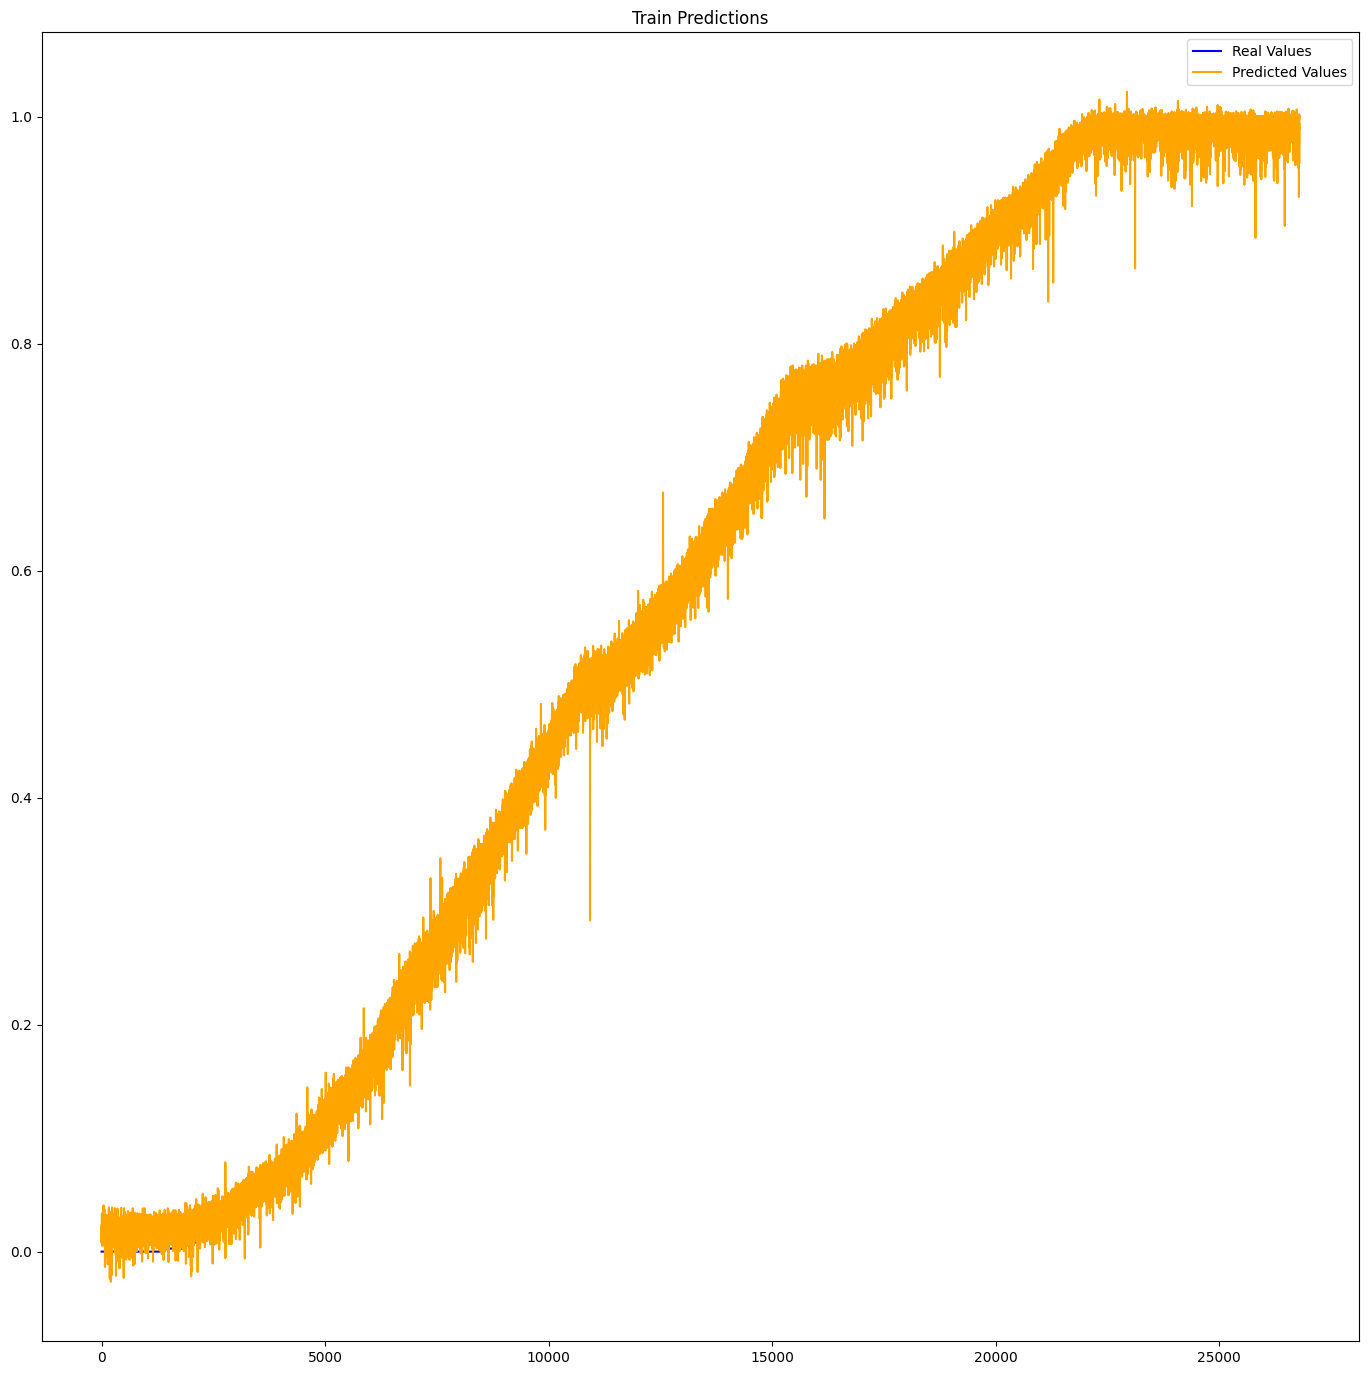
\includegraphics[width=0.35\textwidth]{../Data_Mining_Images/Train_Predictions.png}
	            \caption{MLP - Training Predictions} \label{fig_8}
	        \end{figure}

	       	\textbf{Fig-\ref{fig_8}} shows the training set predictions on the original model. We were able to achive these results in under 25 epochs.
		
		\textbf{Fig-\ref{fig_9}} shows the testing set predictions for the same model. As is evident, the model is able to prdict the target with high accuracy.
		The MSE (Mean-Square-Error) for training was \~ 0.001739, whereas for testing, it was  \~ 0.001731.

  \subsection{\textbf{Results from K-fold cross-validation}}
		\textbf{Fig-\ref{fig_10}} shows result of K-fold validation with k = 5. The scores(MSEs) for all individual folds as well as the mean and standard deviations are consistent with what was expected. Hence, we have succesfully created an MLP based model to answer our domain-specific question and then validated the same using K-fold cross validation.

        \begin{figure*}[!h]
            \centering
            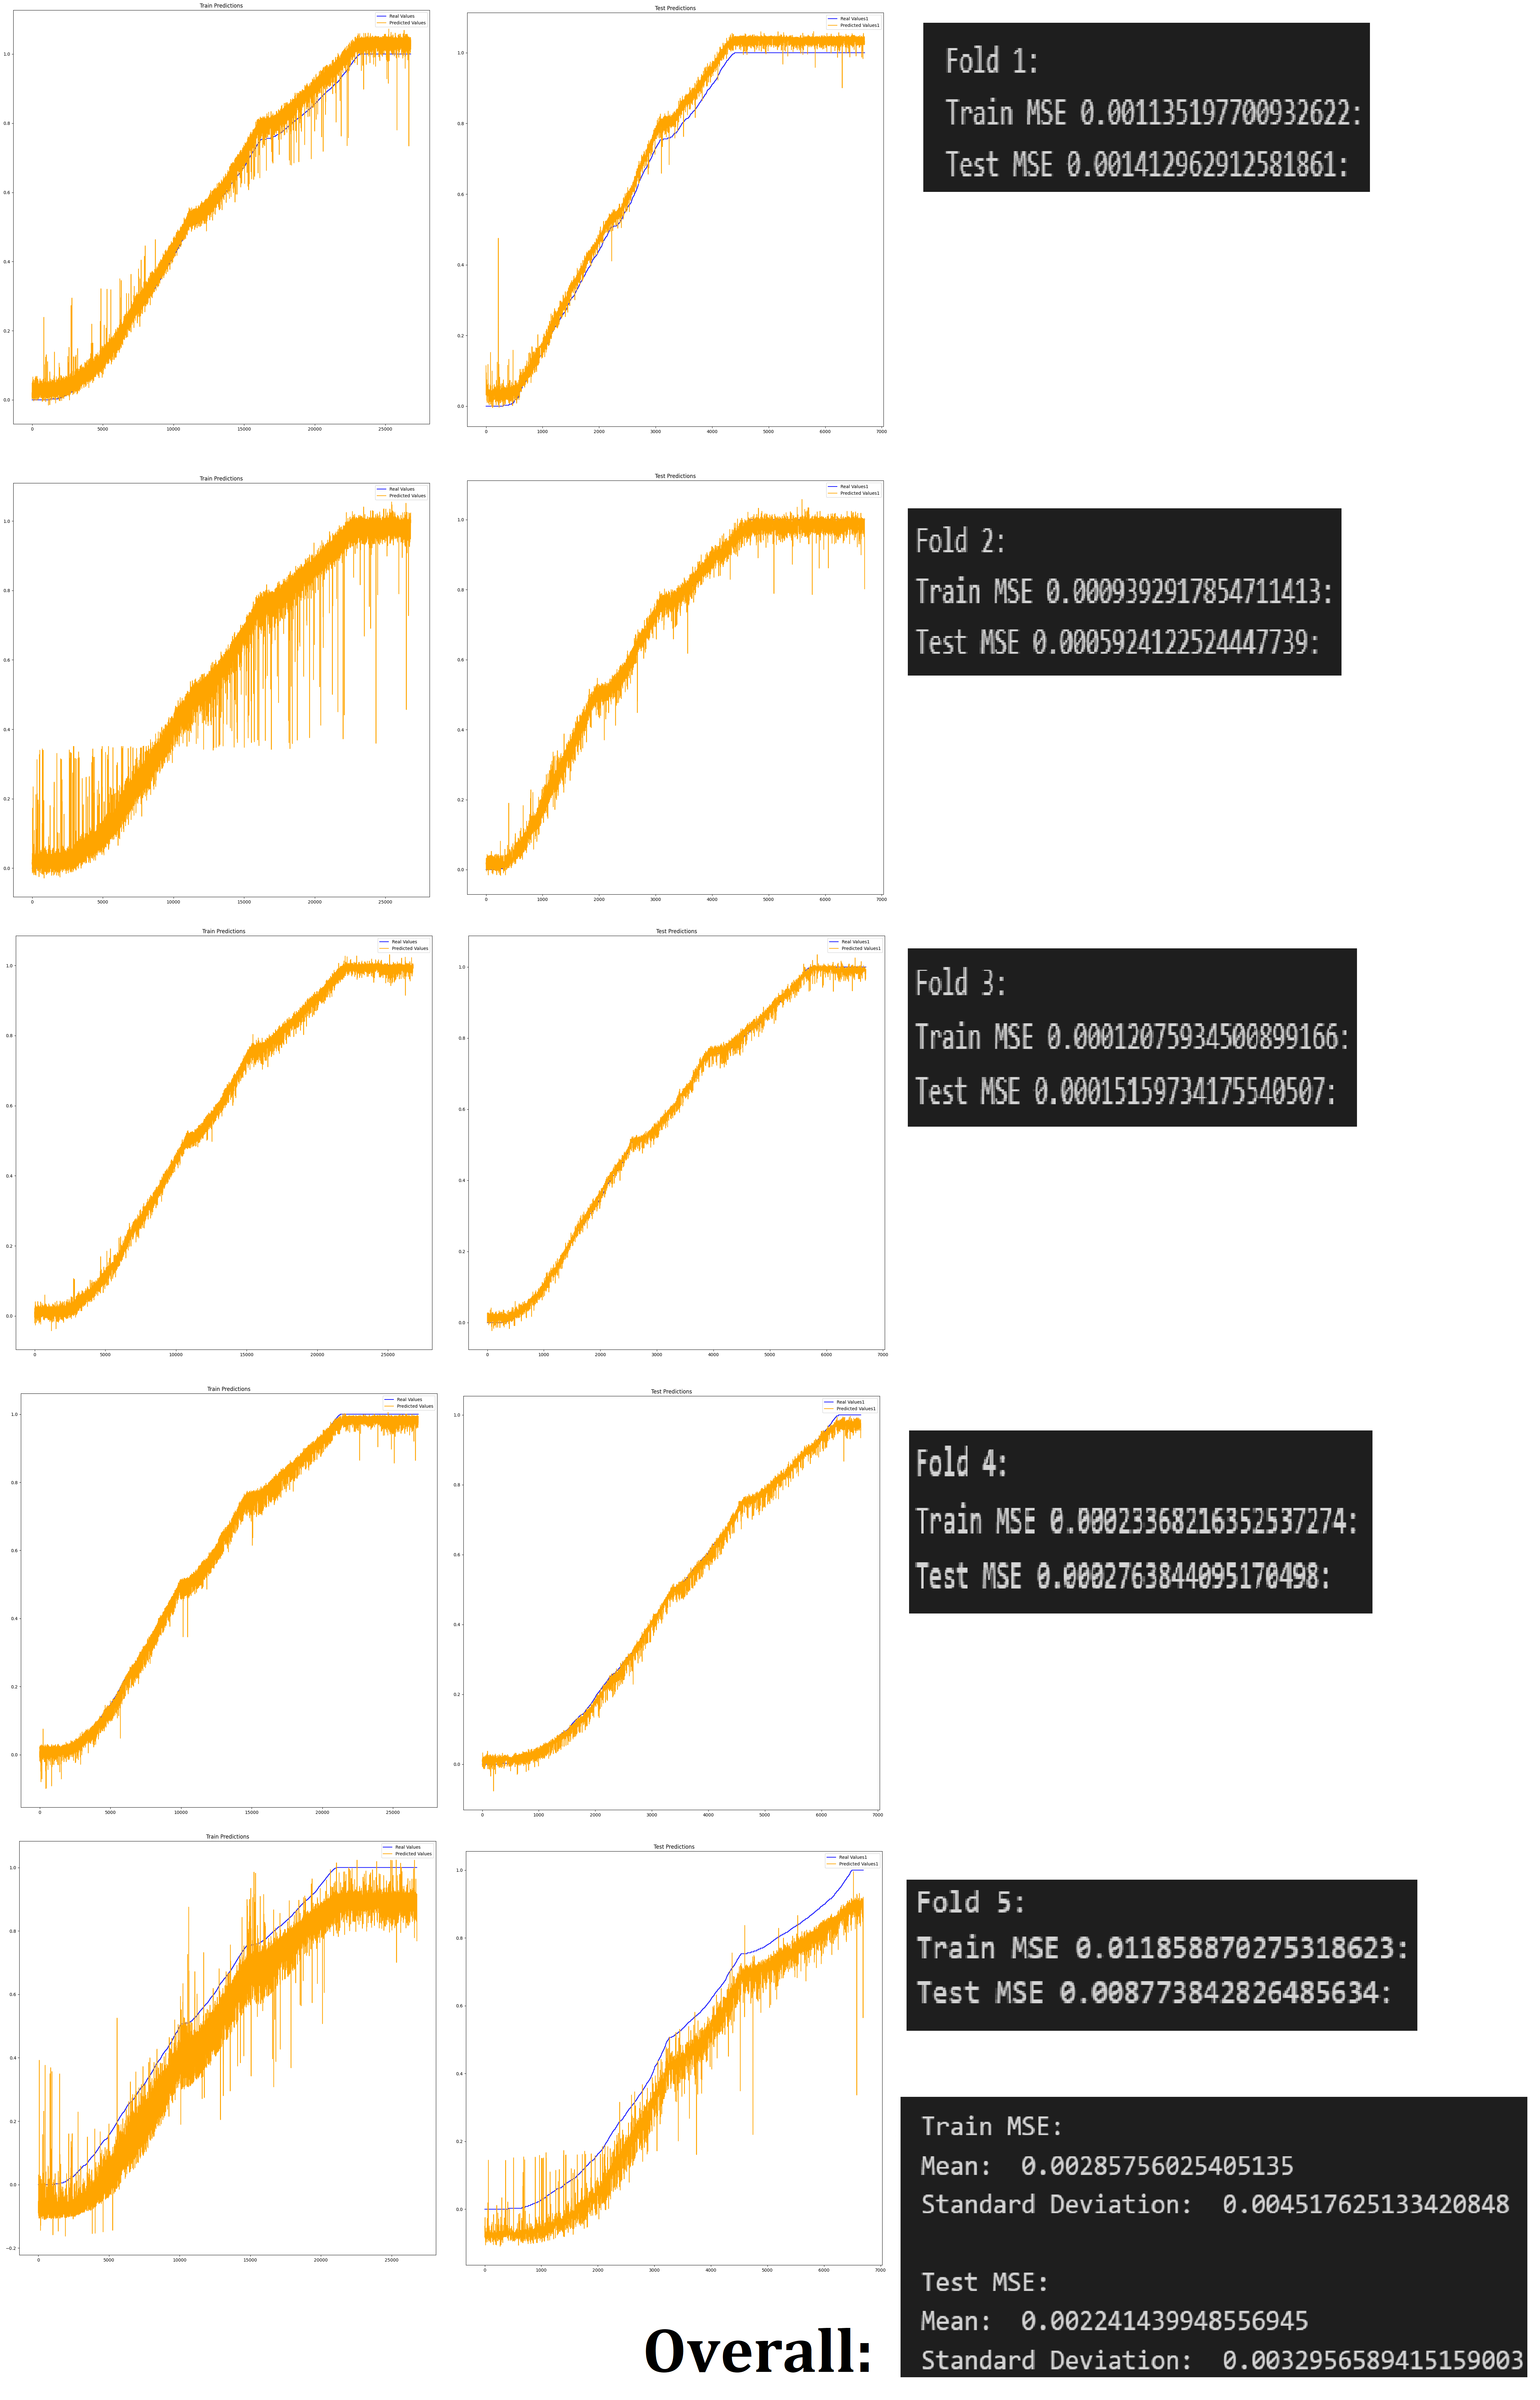
\includegraphics[width=0.8\textwidth]{../Data_Mining_Images/K_Fold_Results.png}
            \caption{K-Fold Validation Results} \label{fig_10}
        \end{figure*}

\newpage
		\begin{figure}[!h]
	            \centering
	            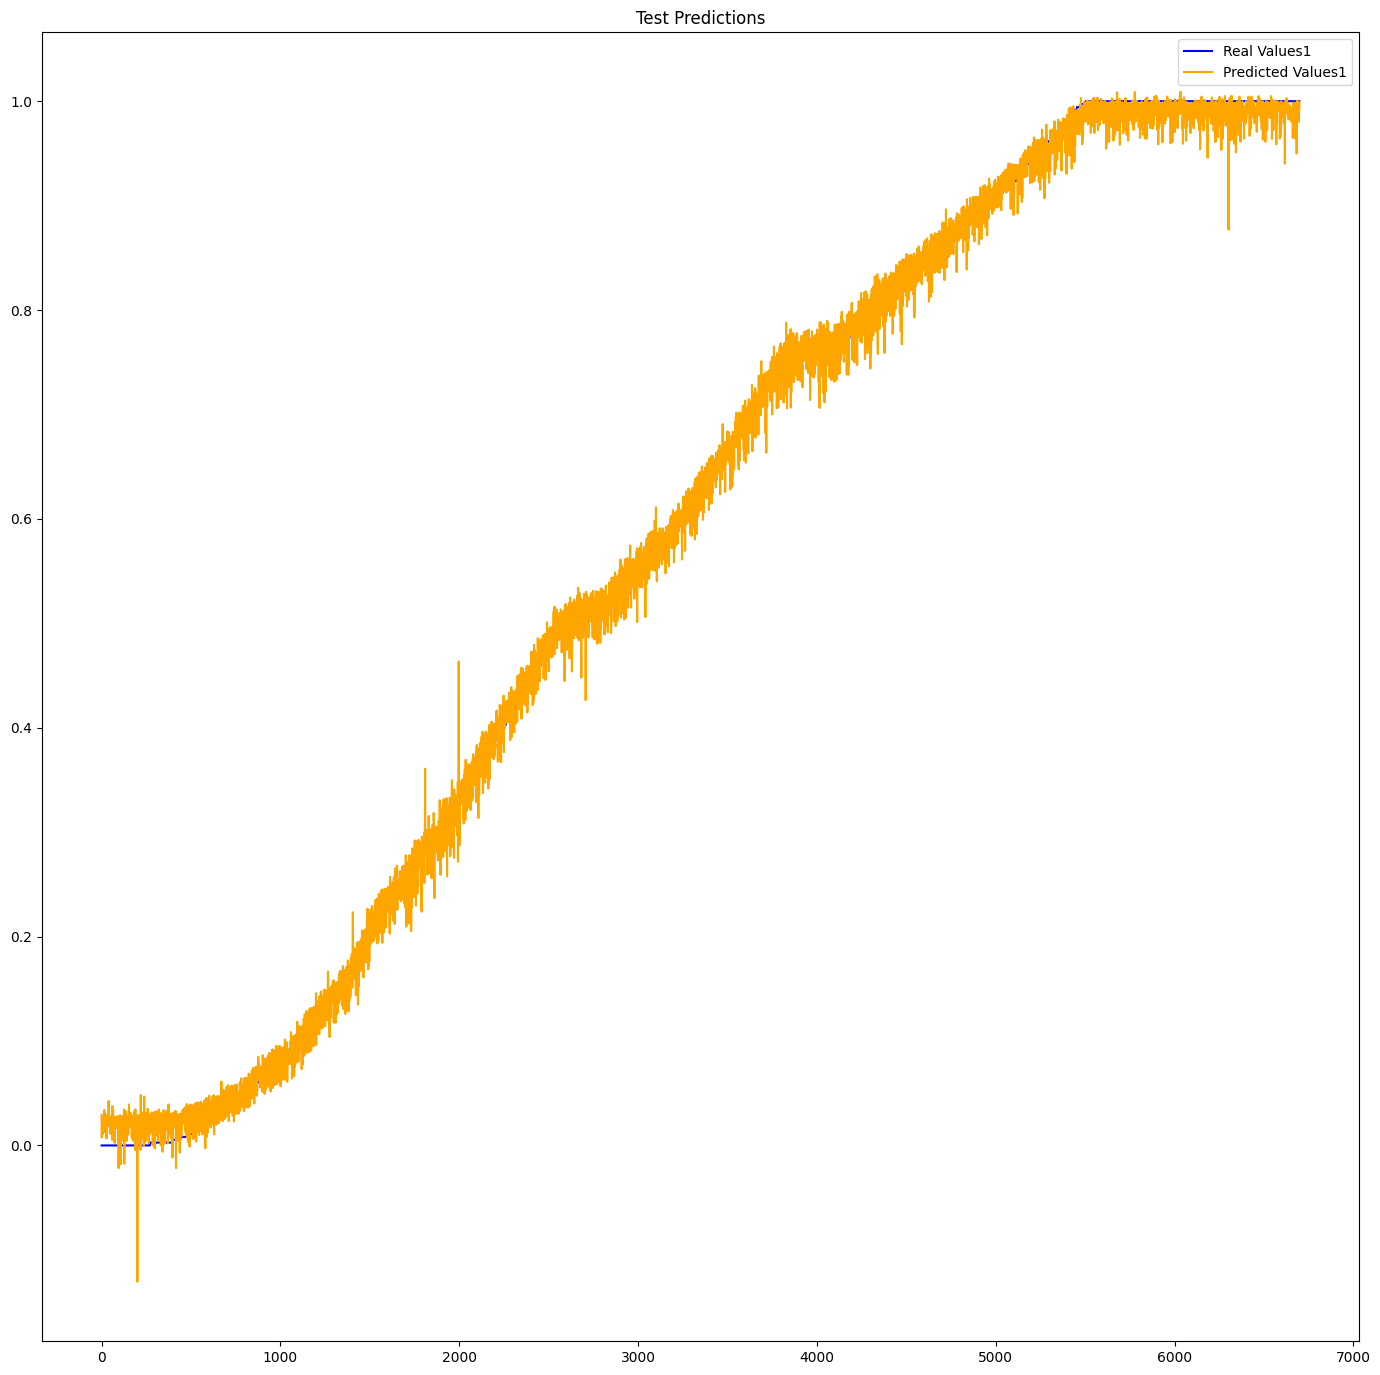
\includegraphics[width=0.35\textwidth]{../Data_Mining_Images/Test_Predictions.png}
	            \caption{MLP - Testing Predictions} \label{fig_9}
	    \end{figure}


\section{\textbf{Final words}}
	\begin{enumerate}
                 \item The features that had been initially proposed have all been implemented using Views, Stored Procedures, REST APIs and the React application.
                 \item The reasons for each of the design choice made for the relational schema have been clearly mentioned in the report in detail.
                 \item The data mining exercise has also been thoroughly discussed in this report. The results achieved after performing K-fold validation were also quite significant.
	      \item For most parts, the report should be the first point of reference, with the video providing a brief of all aspects involved.
	\end{enumerate}


\section{\textbf{Submission}}\label{sec_submission}
	In addition to the submissions made on LEARN, the project submissions can also be found in the following directories:
	\begin{enumerate}
            \item \textit{\small DB Design \& Setup: } {\tiny \url{https://git.uwaterloo.ca/ulaad/backend_travelgenius/-/tree/master/__data__}}
            \item \textit{\small Microservices: } {\tiny \url{https://git.uwaterloo.ca/ulaad/backend_travelgenius}}
            \item \textit{\small Frontend: } {\tiny \url{https://git.uwaterloo.ca/nvtalavi/ece656_frontend}}
	      \item \textit{\small Data Mining: } {\tiny \url{https://git.uwaterloo.ca/ulaad/backend_travelgenius/-/tree/master/__datamining_}}
	\end{enumerate}
	
	\vspace{1mm}

	Access to both repos has been granted on GitLab. Follow the instructions provided in \textbf{Readme.md} in the given sequence, to get the app running on local. There are 2 options for database setup:
	\begin{enumerate}
            \item Marmoset
            \item Local Setup
	\end{enumerate}
	
	\textbf{Readme.md} provides instructions for both. Choose any one as per preference.


\begin{thebibliography}{9}
    \bibitem{1_Airbnb}
        Airbnb, Listings and Review dataset,
        \url {http://insideairbnb.com/get-the-data/}
    \bibitem{2_Email_Regular_Expression}
        Email-Regular Expression, Stack Overflow,
        \url {https://stackoverflow.com/questions/15560004/mysql-check-constraint-for-email-addresses}
    \bibitem{3_Regular_Expression}
        Regular Expression, Regex 101,
        \url {https://regex101.com/}
    \bibitem{4_Backend}
        Database \& Backend Directory, 
        \url{https://git.uwaterloo.ca/ulaad/backend_travelgenius}
    \bibitem{5_Frontend}
        Frontend Directory,
        \url{https://git.uwaterloo.ca/nvtalavi/ece656_frontend}
   \bibitem{6_MLP}
        Tensorflow Keras - MLP
	\url{https://www.tensorflow.org/guide/core/mlp_core}
    \bibitem{7_FeatureSelection}
        Feature Selection with sklearn and Pandas
	\url{https://towardsdatascience.com/feature-selection-with-pandas-e3690ad8504b}
\end{thebibliography}
\vspace{12pt}

\end{document}
